\documentclass[pdflatex,sn-mathphys-num]{sn-jnl}

\usepackage{graphicx}
\usepackage{multirow}
\usepackage{amsmath,amssymb,amsfonts} 
\usepackage{mathtools}
\usepackage{amsthm} 
\usepackage{mathrsfs} 
\usepackage[title]{appendix} 
\usepackage{xcolor} 
\usepackage{textcomp} 
\usepackage{manyfoot} 
\usepackage{booktabs} 
\usepackage{algorithm} 
\usepackage{algorithmicx} 
\usepackage{algpseudocode} 
\usepackage{listings} 
\usepackage{dsfont}
\usepackage{enumerate}   
\usepackage[utf8]{inputenc}
\usepackage{comment}
\usepackage{adjustbox}  
\usepackage{geometry}   
\usepackage{rotating}
\usepackage{subcaption}
\usepackage{array}
\usepackage{upgreek}
\usepackage{tikz}
\usetikzlibrary{shapes, arrows, positioning, fit}

\newcommand{\reals}{\mathbb{R}}
\newcommand{\nats}{\mathbb{N}}
\newcommand{\Prob}{\mathbb{P}}
\newcommand{\E}{\mathbb{E}}
\newcommand{\Var}{\mathbb{V}\text{ar}}
\newcommand{\Cov}{\mathbb{C}\text{ov}}
\newcommand{\Norm}{\mathcal{N}}
\newcommand{\Gam}{\text{Gamma}}
\newcommand{\ind}{\mathds{1}}
\newcommand{\Corr}{\,\text{Corr}}
\newcommand{\natsstar}{\mathbb{N}^*}
\newcommand{\textopt}{\text{opt}}
\newcommand{\textMH}{\text{MH}}
\newcommand{\texte}{\text{e}}
\newcommand{\ones}{\mathbf{1}} 

\DeclareMathOperator*{\argmax}{\arg\!\max}
\DeclareMathOperator*{\argmin}{\arg\!\min}
\DeclareMathOperator*{\cart}{\bm{\times}}

\renewcommand{\geq}{\geqslant}
\renewcommand{\leq}{\leqslant}

\theoremstyle{thmstyleone} 
\newtheorem{theorem}{Theorem} 
\newtheorem{lemma}{Lemma}
\newtheorem{proposition}{Proposition}  
\newtheorem{corollary}{Corollary}

\theoremstyle{thmstyletwo} 
\newtheorem{example}{Example} 
\newtheorem{remark}{Remark} 


\theoremstyle{thmstylethree} 
\newtheorem{definition}{Definition} 
\newtheorem{hypothesis}{Assumption} 

\raggedbottom

\begin{document}

\title[Article Title]{Adaptive Pseudo-Marginal Algorithm}

\author*[1]{\fnm{Sarra} \sur{Abaoubida}}\email{sarra.abaoubida@umontreal.ca}

\author[1]{\fnm{Mylène} \sur{Bédard}}

\author[1]{\fnm{Florian} \sur{Maire}}

\affil*[1]{\orgname{Université de Montréal}, \orgdiv{Département de mathématiques et statistique}} 

\abstract{The Pseudo-Marginal (PM) algorithm is a popular Markov chain Monte Carlo (MCMC) method used to sample from a target distribution when its density is inaccessible, but can be estimated with a non-negative unbiased estimator. Its performance depends on a key parameter, \textit{N}, the number of iterations (or particles) used to approximate the target density. Larger values of \textit{N} yield more accurate estimates but at increased running time. Previous studies has provided guidelines for selecting an optimal value of \textit{N} to balance this tradeoff. However, this approach involves multiple steps and manual adjustments.
To overcome these limitations, we introduce an adaptive version of the PM algorithm, where \textit{N} is automatically adjusted during the iterative process toward its optimal value, thus eliminating the need for manual intervention. This algorithm ensures convergence under certain conditions. On two examples, including a real data problem on pulmonary infection in preschool children, the proposed algorithm compares favorably to the existing approach.}

\keywords{Adaptive Markov chain Monte Carlo, Intractable likelihood, Ergodicity}

\maketitle

\section{Introduction}
\label{sec:intro}
In a Bayesian context, we consider a model where the likelihood function of the observations $y \in \mathcal{Y}^T$ is denoted by $p_T(y \lvert \theta)$, and the prior distribution of the parameter \mbox{$\theta\in\Theta\subseteq\mathbb{R}^d
$} has density $p(\theta)$. Consequently, the posterior density is \mbox{$\pi(\theta) \propto p_T(y \lvert \theta) p(\theta)$}. In this context, the fundamental statistical task reduces to computing posterior expectations of the form $ \pi(f) := \E[f(\theta)|y] = \int f(\theta) \pi(\mathrm{d}\theta),$ for measurable functions $f$ satisfying $\pi(f^2) < \infty$. An approximation of this posterior expectation is easily accessible from a MCMC sampler, via the sample average $\widehat{\pi}_L(f) = L^{-1}\sum_{\ell=0}^{L-1} f(\theta_\ell)$ obtained from the Markov process $\{\theta_\ell, \ell\geq 0\}$. A widely used MCMC method is the Metropolis-Hastings (MH) algorithm, which generates a Markov chain with stationary distribution $\pi(\theta)$. At each step, given the current state $\theta$, a candidate $\vartheta$ is proposed, and then accepted with a probability that typically depends on the likelihood ratio $p_T(y \lvert \vartheta)/p_T(y \lvert \theta)$. However, in many statistical models, direct computation of the likelihood \( p_T(y|\theta) \) is challenging, rendering the standard MH impractical.

The PM algorithm, introduced in \cite{andrieu_convergence_2015} and formally described in Section~\ref{sec:pm}, overcomes this by replacing the intractable likelihood ratio $p_T(y \lvert \vartheta)/p_T(y \lvert \theta)$ with an unbiased non-negative estimator. Standard approaches like importance sampling (using weighted observations) and particle filtering (for state-space models) generate such estimators by averaging over $N$ realizations. Substituting the true likelihood with an estimate in the MH introduces a trade-off: as \( N \) increases, the asymptotic accuracy of a PM chain improves, but at a higher computational cost (runtime). Therefore, a key challenge is balancing computational efficiency and statistical accuracy. The weak convergence properties of the PM algorithm were explored in \cite{schmon_large-sample_2021}, providing guidelines for choosing the optimal number of Monte Carlo samples/particles \( N \) to use in the PM, based on the dimension \( d \) of the parameter $\theta$. However, this approach requires manual tuning and sequential execution of multiple steps. We summarize this non adaptive method in Section~\ref{sec:review}.

In Section~\ref{sec:APM}, we propose an efficient alternative by letting $N$ evolve over the iterations of the PM algorithm, allowing it to approach its optimal value automatically. This scheme follows the same steps as in \cite{schmon_large-sample_2021} but integrates them into a single process, leading to the Adaptive Pseudo-Marginal (APM) algorithm. By doing so, we naturally lose the Markov property of the process because the adjustment of $N$ depends on the entire history of the chain. It is thus important to verify that our adapted sampler converges to the target distribution. As specified in \cite{roberts_coupling_2007}, two conditions ensure the convergence of an adaptive algorithm to the target distribution: the \textit{diminishing adaptation} and the \textit{containment condition}.

The APM we propose satisfies the \textit{diminishing adaptation} by construction, allowing $N$ to adapt with a probability that decreases gradually to zero over the iterations. Furthermore, in Section~\ref{sec:APM}, we establish theoretical conditions under which the APM satisfies the \textit{containment condition}. These conditions rely on the polynomial ergodicity of the PM algorithm and convex ordering of the likelihood estimations. We show that the APM marginally converges to the posterior distribution in terms of total variation distance under these assumptions.

In Section~\ref{sec:syntheticex}, we rigorously compare the performance of the APM against the non adaptive approach in \cite{schmon_large-sample_2021}, using a synthetic example with simulated data. We prove that the model specified in this example satisfies the theoretical conditions established in Section~\ref{sec:APM} for the convergence of the APM. Our simulations show that the computational cost of the proposed adaptive method is significantly lower than that of its non adaptive counterpart, highlighting its practical advantages. Finally, in Section~\ref{sec:realex}, the performance of the APM is evaluated on real data from \cite{zeger_generalized_1991} and compared to the non adaptive approach. Empirically, both methods yield identical posterior means and variances with comparable runtimes. However, the APM remains advantageous by allowing dynamic adaptation of \( N \), eliminating the need for manual tuning.



\section{The Pseudo-Marginal Algorithm}
\label{sec:pm}
Prior to formalizing the PM framework, we begin by recalling the standard MH algorithm, which generates a Markov chain with stationary distribution $\pi(\theta)$. The transition kernel of the MH takes the form:
\begin{align*}
P(\theta, d\vartheta) = q(\vartheta|\theta)\min\left\{1,r(\theta,\vartheta)\right\}d\vartheta + \left(1-\int_\Theta q(\vartheta|\theta)\min\left\{1,r(\theta,\vartheta)\right\}d\vartheta\right)\delta_\theta(d\vartheta),
\end{align*}
where $\vartheta \mapsto q(\vartheta|\theta)$ is the proposal density and where the acceptance ratio, $r(\theta,\vartheta)={p_T(y|\vartheta)p(\vartheta)q(\theta|\vartheta)}/\{p_T(y|\theta)p(\theta)q(\vartheta|\theta)\} \label{MHratio}$, depends crucially on the likelihood evaluation. 

As mentioned in Section~\ref{sec:intro}, if \(p_T(y|\theta) \) is intractable, the MH algorithm becomes infeasible. A powerful approach addressing this problem is the PM algorithm where the key innovation is to replace the exact likelihood with an unbiased, non-negative estimator $\widehat{p}_{N,T}(y|\theta,U)$ in the MH acceptance ratio, with $U|\theta \sim m_{N,\theta}(\cdot)$ the auxiliary variables used to compute the likelihood estimator (see \cite{lin_noisy_2000, beaumont_estimation_2003, andrieu_pseudo-marginal_2009}). 

To understand the theoretical foundation of the PM, consider the extended target distribution:
\begin{align}
\bar{\pi}_N(\theta,u) = \pi(\theta)m_{N,\theta}(u)\frac{\widehat{p}_{N,T}(y|\theta,u)}{p_T(y|\theta)}.
\label{pmpost}
\end{align}
Since $\widehat{p}_{N,T}(y \lvert \theta, U)$ is unbiased, this extended target admits $\pi$ as its marginal distribution by construction. The PM algorithm is a MH algorithm targeting (\ref{pmpost}) with proposal density 
$(\vartheta , v) \mapsto q(\vartheta\lvert\theta) m_{N,\vartheta}(v)$. 
The acceptance probability for a candidate $(\vartheta, v)$ is thus given by
\begin{align}
    \alpha_N\left(\theta,u ;  \vartheta,v\right) 
    &=\min \left\{1, \frac{\widehat{p}_{N,T}(y \lvert \vartheta, v) p(\vartheta) q(\theta \lvert \vartheta)}{\widehat{p}_{N,T}(y \lvert \theta, u) p(\theta) q(\vartheta \lvert\theta)}\right\}.
    \label{alphaN}
\end{align}
The PM acceptance ratio does not depend on the intractable true likelihood, making $\alpha_N$ computable. This shows that while PM algorithms are approximations of \(P\), they are exact in the sense that, at equilibrium, they sample marginally from the desired distribution \( \pi \). The transition kernel of the PM algorithm is given by
\begin{align}
    P_N(\theta, u; d\vartheta, dv) &= q(\vartheta \lvert \theta) m_{N,\vartheta}(v) \alpha_N(\theta, u; \vartheta, v) d\vartheta dv + \varrho_{N}(\theta, u) \delta_{(\theta, u)}(d\vartheta, dv),
\label{equa4}
\end{align}
where 
\begin{equation}
    \varrho_{N}(\theta, u) =  1 - \int
        _{\Theta \times \mathcal{U}} q(\vartheta \lvert \theta)m_{N,\vartheta}(v) \alpha_N(\theta, u; \vartheta, v) d\vartheta dv,
        \label{varrho}
\end{equation}
and $\delta_{(\theta, u)}$ is the Dirac measure at $(\theta, u)$. 

Following the work of \cite{andrieu_pseudo-marginal_2009, pitt_properties_2012, andrieu_convergence_2015,doucet_efficient_2015, sherlock_efficiency_2015, andrieu_establishing_2016, schmon_large-sample_2021}, we turn to a more abstract reparameterization of the PM algorithm. We introduce the weight $W_N(\theta) = \widehat{p}_{N,T}(y|\theta,U)/p_T(y|\theta)$, which we view as a multiplicative perturbation, or noise, of the true likelihood $p_T(y|\theta)$ since  $\widehat{p}_{N,T}(y|\theta, U)=p_T(y|\theta) W_N(\theta)$. Now, let $\left\{\mathcal{Q}_{N,\theta}\right\}_{\theta \in \Theta}$ be a family of probability measures on the positive reals $\left(\mathbb{R}_{+}^{*}, \mathcal{B}\left(\mathbb{R}_{+}^{*}\right)\right)$ indexed by $\theta \in \Theta$ and such that $\E[W_N(\theta)]=\int w \mathcal{Q}_{N,\theta}(\mathrm{d} w)=1$ for any $\theta \in \Theta$. One can check that the Markov transition probability ${P_N}$ of the PM approximation of the marginal kernel $P$ is a MH algorithm targeting 
$$\bar{\pi}_N(\theta, \mathrm{d} w)= \pi(\theta) \mathcal{Q}_{N,\theta}(\mathrm{d} w) w.$$
For any $(\theta, w) \in \Theta \times \mathcal{W}$ (with $\mathcal{W}:=(0, \infty))$, this kernel can be expressed as
\begin{align}
{P_N}(\theta, w ; \mathrm{d} \vartheta,\mathrm{d} z)= & q(\vartheta|\theta) \min \left\{1, r(\theta, \vartheta) \frac{z}{w}\right\} \mathcal{Q}_{N,\vartheta}(\mathrm{d} z) \mathrm{d}\vartheta + {\rho_N}(\theta, w)\delta_{\theta, w}(\mathrm{d} \vartheta ,\mathrm{d} z) ,
\label{equa5}
\end{align}
where the rejection probability is
\begin{align}
     \varrho_{N}(\theta, w) = 1- \int
    _{\Theta \times \mathcal{W}} q(\vartheta|\theta) \min\left\{1,  r(\theta, \vartheta) \frac{z}{w}\right\}
    \mathcal{Q}_{N,\vartheta}(\mathrm{d}z) \mathrm{d}\vartheta.
\label{varrho_repar}
\end{align}

The acceptance ratio in the PM algorithm can be viewed as a multiplicative perturbation of the standard MH acceptance ratio. Although the weights $W_N(\theta)$ fundamentally influence the transition kernel, they are not explicitly computed in practical implementations. This is because the PM algorithm operates directly with the likelihood estimators $\widehat{p}_{N,T}(y | \theta, U)$ in the acceptance ratio \eqref{alphaN}, completely bypassing evaluation of the intractable true likelihood $p_T(y | \theta)$. In their analysis, several authors \cite{schmon_large-sample_2021, pitt_properties_2012, doucet_efficient_2015, sherlock_efficiency_2015, deligiannidis_correlated_2018} refer to the quantity $\log\{W_N(\theta)\}$ as the additive noise or the log-likelihood error, and derive several theoretical results by reparameterizing the PM algorithm in terms of this noise.

Having formally introduced the PM algorithm, we now review previous articles examining the critical role of the Monte Carlo parameter (or number of particles) \( N \) in governing its performance. In conventional Monte Carlo methods \cite{robert_monte_2004}, increasing \( N \) improves estimator accuracy at the expense of computational effort, creating a fundamental trade-off between statistical precision and runtime, a trade-off that also applies to the PM context. To properly evaluate this trade-off and compare the PM algorithm variants, we discuss in Section~\ref{sec:review} an appropriate efficiency measure, namely the computing time (see \cite{pitt_properties_2012,doucet_efficient_2015,schmon_large-sample_2021}). We then present the non adaptive method of \cite{schmon_large-sample_2021}, which implements the PM with the optimal value of \(N\).

\section{Computing Time Optimization in Pseudo-Marginal Algorithms}
\label{sec:review}
Following \cite{pitt_properties_2012, doucet_efficient_2015, schmon_large-sample_2021}, we adopt the computing time (CT) measure to balance statistical precision and computational cost (runtime).  Formally defined in (\ref{CT}), this metric quantifies the trade-off between asymptotic variance (\ref{asympvar}) and computational cost, ensuring efficient resource allocation when minimized.

As discussed in Section~\ref{sec:intro}, Bayesian inference often requires estimating an expectation $\pi(f)$ using an empirical average $\widehat{\pi}_L(f)$. The latter is computed from a Markov chain $\{\theta_\ell, \ell \geq 0\}$ generated by a transition kernel $Q$. The efficiency of this approximation is closely linked to the mixing properties of $Q$, with well-designed algorithms leading to estimators that feature low asymptotic variances. Under mild conditions (see \cite{haggstrom_variance_2007}) and for $f \in L^2(\pi)$, the asymptotic variance of an MCMC estimator is finite and given by
\begin{align}
    \overline{\Var}(f, Q) &= \lim_{L \rightarrow \infty} \frac{1}{L} \E \left[\left(\sum_{\ell=0}^{L-1} f(\theta_\ell) - \pi(f)\right)^2 \right] 
    = \Var(f(\theta_0)) \operatorname{IF}(f, Q),
    \label{asympvar}
\end{align}
where the inefficiency factor 
\begin{equation}
    \operatorname{IF}(f, Q) = 1 + 2\sum_{\ell=1}^{\infty}\frac{\Cov(f(\theta_0),f(\theta_\ell))}{\Var(f(\theta_0))} < \infty
    \label{inefficiency}
\end{equation}
is a measure of how much the estimator is penalized by the correlation induced by the Markov chain.

Theorem 10 in \cite{andrieu_establishing_2016} establishes that for likelihood estimators obtained via importance sampling, the asymptotic variance of the PM algorithm decreases as the number of Monte Carlo samples \(N\) increases. However, larger values of \(N\) incur higher computational costs. The goal is thus to find the optimal value of $N$, that is a value that balances the computational cost and the asymptotic variance of the estimator $\widehat{\pi}_L(f)$. 

A solution to this optimization problem was first proposed in \cite{pitt_properties_2012} and further refined in \cite{doucet_efficient_2015, sherlock_efficiency_2015, schmon_large-sample_2021}, where results are derived under two key assumptions:
\begin{enumerate}[(i)]
    \item The additive noise satisfies $\omega_N(\theta) := \log\{W_N(\theta)\} \sim \mathcal{N}(-\sigma^2/2, \sigma^2)$ for all $\theta \in \Theta$, with $\sigma^2$ constant with respect to $\theta$.
    \label{hypi}
    \item The variance of the additive noise scales as $\sigma^2 \propto 1/N$.
    \label{hypii}
\end{enumerate}
\begin{remark}
    Assumption~\eqref{hypii} was demonstrated by \cite{ deligiannidis_correlated_2018, berard_lognormal_2014} in the large sample regime ($T \to \infty$).
\end{remark}

Under assumptions (\ref{hypi}) and (\ref{hypii}), \cite{pitt_properties_2012} proposed optimizing the additive noise standard deviation \(\sigma\) by minimizing the computing time (CT) of the PM chain. This quantity is defined, for functions $\bar f \in L^2(\bar{\pi}_N)$, as:
\begin{equation}
    \text{CT}(\bar f,P_\sigma) :=  \frac{\operatorname{IF}(\bar f,P_\sigma)}{\sigma^2} \propto \frac{\overline{\Var}(\bar f,P_\sigma)}{\sigma^2},
    \label{CT}
\end{equation}
where the transition kernel $P_\sigma$ of the PM chain becomes, under Assumption \eqref{hypi},
\begin{align}
   {P_\sigma}\left(\theta,\omega ; \mathrm{d} \vartheta,\mathrm{d}\zeta\right)&= q(\vartheta|\theta) \varphi(\zeta ; -\sigma^2/2, \sigma^2) \min \left\{1, r(\theta, \vartheta) \exp\{\zeta-\omega\}\right\}  \mathrm{d}\vartheta \mathrm{d}\zeta \nonumber\\*
   &\quad +  {\rho_\sigma}(\theta,\omega) \delta_{\theta, \omega}(\mathrm{d} \vartheta ,\mathrm{d}\zeta),
   \label{limitkernel}
\end{align}
with \({\rho_\sigma}(\theta,\omega)\) representing the rejection probability and $\varphi(x; \mu, \sigma^2)$ the density of a $\Norm(\mu,\sigma^2)$ evaluated at $x$. The value of CT is thus affected by the interplay between computational cost, which scales as $1/\sigma^2 \propto N$ (the number of particles used to compute the unbiased estimator), and the inefficiency factor $\operatorname{IF}(\bar{f},P_\sigma)$.

Under this framework, the authors in \cite{schmon_large-sample_2021} generalized the work of \cite{doucet_efficient_2015, sherlock_efficiency_2015, pitt_properties_2012} and obtained a weak convergence result for the PM chain \(P_N\) as the dataset size \(T \to \infty\). Specifically, under appropriate regularity conditions, they demonstrated that a properly rescaled PM chain converges weakly to a limiting PM chain targeting a Normal distribution. In this limiting regime, the transition kernel $P_\sigma$ satisfies \eqref{limitkernel} and the additive noise follows a Normal distribution with constant mean and variance, as assumed in (\ref{hypi}); we refer the reader to Section 3 in \cite{schmon_large-sample_2021} for a precise definition of this weak convergence result.

Based on the limiting chain $P_\sigma$ in~\eqref{limitkernel} and using the Normal random walk proposal density
\[
q(\vartheta|\theta) = \varphi\left(\vartheta; \theta, \frac{l^2}{d} I_d\right),
\]
where the scaling $l^2/d$ follows the framework in~\cite{sherlock_efficiency_2015}, the authors in~\cite{schmon_large-sample_2021} obtained the optimal values $(l_{\text{opt}}, \sigma_{\text{opt}})$ that minimize the computing time $\mathrm{CT}(\bar f, P_\sigma)$ defined in~\eqref{CT}. To obtain these values, they considered optimizing under the function $\bar f(\theta, \omega_N(\theta)) = \theta_1$, where $\theta_1$ denotes the first coordinate of $\theta$. For each dimension $d$, they ran multiple chains over a finely spaced grid of candidate values for $(l, \sigma)$, computed the corresponding computing times for each pair, and then selected the pair $(l_{\text{opt}}, \sigma_{\text{opt}})$ that yielded the minimum computing time. The resulting optimal tuning parameters were reported for various values of $d$ (see Table~1 in~\cite{schmon_large-sample_2021}).

Following these observations, \cite{schmon_large-sample_2021} proposed a method of implementation the PM algorithm with the optimal number of particles, $N_{\text{opt}}$. After using Table 1 in \cite{schmon_large-sample_2021} to identify the estimated optimal scaling parameter $l_\text{opt}$ and additive noise standard deviation $\sigma_\text{opt}$ as a function of the parameter dimension $d$, this method can be summarized as follows:
\begin{enumerate}
    \item Run a preliminary PM algorithm with some initial $N_1$ to obtain $\hat \theta_{N_1}$ and $\widehat \Sigma_{N_1}$, the posterior mean and covariance estimates of $\theta$. At this stage, the proposal density is a Normal random walk with covariance ${l_{\text{opt}}^2 \Sigma_p}/{d}$, where $\Sigma_p$ is some positive-definite matrix.
    \label{step1}

    \item Let $\sigma_N^2(\hat \theta_{N_1})$ denote the variance of the additive noise $\omega_N(\hat \theta_{N_1})$, defined as:
    \begin{align}
        \sigma_N^2(\hat \theta_{N_1}) &= \Var(\omega_N(\hat \theta_{N_1})|\hat \theta_{N_1})\nonumber \\
        &= \Var\big(\log\{\widehat p_N(y |\hat \theta_{N_1}, \widehat U)\}- \log\{p_N(y |\hat \theta_{N_1})\}\big|\hat \theta_{N_1}\big) \nonumber\\
        &= \Var\big(\log\{\widehat p_N(y |\hat \theta_{N_1}, \widehat U)\}|\hat \theta_{N_1}\big),
        \label{estimationsd}
    \end{align}
    where the auxiliary variables $\widehat U|\hat\theta_{N_1} \sim m_{N, \hat \theta_{N_1}}$. 
    We estimate $\sigma_N^2(\hat \theta_{N_1})$ via Monte Carlo methods for multiple values of $N$ and select $N_{\text{opt}}$ such that the variance estimate of the additive noise, $\hat \sigma_{N_{\text{opt}}}^2(\hat \theta_{N_1})$, matches the target value $\sigma_{\text{opt}}^2$. 
    This step is facilitated by the inverse proportionality between $1/\sigma^2$ and $N$, as stated in Assumption~\eqref{hypii}. Thanks to this relationship, one can choose a reasonable interval for $N$ and efficiently narrow down the search, as the approximate location of the optimal $N$ can be anticipated.
    \label{step2}
    
    \item Execute the PM algorithm using $N_{\text{opt}}$ and a Normal random walk proposal density with covariance ${l_{\text{opt}}^2\widehat \Sigma_{N_1}}/{d}$.
    \label{step3}
    \label{NAmethod}
\end{enumerate}

\begin{remark}
        Choosing an excessively large value for \( N_1 \) may lead to unnecessary computational burden, while a value too small may yield inaccurate estimates of \( \hat\theta_{N_1} \) and \( \hat\sigma_{N_1} \), thereby degrading the performance of subsequent steps.
\end{remark}
\begin{remark}
Step~\ref{step2} is typically carried out via manual tuning of the number of particles \( N \), by iteratively adjusting \( N \) and visually inspecting the resulting variability of the additive noise. However, such trial-and-error procedures are inherently subjective, difficult to automate, and complicate reproducibility. To overcome these limitations, we employ a principled and automated approach based on a \emph{dichotomic search} algorithm (see Subsection~\ref{dichotomic}), which iteratively narrows the search interval until a predefined precision \( a_1 \) is achieved. This method ensures consistent selection of \( N_{\text{opt}} \) across independent runs, while also enabling precise measurement of runtime, which facilitates a direct comparison with the APM algorithm introduced in Section~\ref{sec:APM}.
\end{remark}

This non adaptive approach requires multiple steps, each of which must be executed sequentially, making the process somewhat time-consuming and adding a cognitive load. We propose an efficient alternative to this approach by combining these three steps into a single process, in which we allow the parameter $N$ to gradually approach its optimal value as the PM iterations progress using an adaptive scheme. Both methods will then be rigorously compared using synthetic and real data. 

\section{The Adaptive Pseudo-Marginal Algorithm}
\label{sec:APM}
In adaptive MCMC methods, tuning parameters (e.g., proposal variance) are often updated using \textit{epoch-based strategies} to ensure computational stability (see \citep{roberts_examples_2009, haario_adaptive_2001}). An \textit{epoch} is a series of $K$ consecutive MCMC states, \( \{\theta_{\ell-K+1}, \dots, \theta_\ell\} \), during which no adaptation occurs. After each \textit{epoch}, empirical statistics (e.g., mean, covariance, or acceptance rate) are computed from the samples in that \textit{epoch}. These statistics serve as inputs to an \textit{adaptation criterion}, for example, comparing the observed acceptance rate to an optimal value (like 0.234 for the Random Walk Metropolis (RWM), \cite{gelman_weak_1997}). If the criterion suggests suboptimal performance, the algorithm adjusts its parameters before proceeding to the next \textit{epoch}. This periodic adjustment balances adaptation with stability.

In this section, we introduce our adaptive version of the PM algorithm, called APM, where the parameter $N$, used in the estimation of \( \widehat{p}_{N,T}(y | \theta, U) \), evolves according to a \textit{epoch-based adaptation strategy}. As discussed in Section~\ref{sec:review}, Table~1 in \cite{schmon_large-sample_2021} provides explicit values for the optimal standard deviation of the additive noise $\sigma_{\text{opt}}$ as a function of parameter dimension $d$. During sampling, the APM periodically computes an empirical estimate \( \hat{\sigma}^2_\ell \) of the additive noise variance after every \textit{epoch} of size \( K \). This occurs at iterations \( \ell = K j \), where \( j \in \nats^*\) is the \textit{epoch} index. By comparing $\hat{\sigma}_\ell^2$ to $\sigma^2_{\text{opt}}$, the APM adjusts $N$ with step size $a \in \nats^*$ after each \textit{epoch}. The inverse proportionality between $\sigma^2$ and $N$ directly motivates our adaptive framework: increasing \( N \) reduces \( \sigma \), while decreasing \( N \) inflates it, which allows us to steer $\sigma$ toward $\sigma_\textopt$.
 
Let $N_\ell$ be an $\mathbb{N}^*$-valued random variable controlling the transition kernel at iteration $\ell$. The state of the algorithm at this iteration is given by the $\Theta \times \mathcal{W}$-valued random variable $(\theta_\ell, W_\ell)$, where $W_\ell= W_{N_{\ell-1}}(\theta_\ell)$ is the weight introduced in Section~\ref{sec:pm}. The filtration $\mathcal{G}_\ell = \sigma(\theta_0, W_0, N_0, \ldots, \theta_\ell, W_\ell, N_\ell)$ encodes the full history of the algorithm up to iteration $\ell$. The transition dynamics satisfy
\begin{align}
    \mathbb{P}\left[(\theta_{\ell+1}, W_{\ell+1}) \in A |\mathcal{G}_\ell\right] = P_{N_\ell}(\theta_\ell, W_\ell; A) = P_{\psi(N_{\ell-1}, \hat\sigma_\ell)}(\theta_\ell, W_\ell; A),
    \label{adaptivetransition}
\end{align}
where $P_{N_\ell}$ is the PM transition kernel defined in equation~(\ref{equa5}), and $\psi$ is the adaptation function given by
\begin{align*}
\psi(N_{\ell-1}, \hat{\sigma}_\ell) = N_{\ell-1} + a \cdot \kappa_\ell (\hat\sigma_\ell) \cdot \ind(\ell \in K\nats^*),
\end{align*}
with step size \( a \in \natsstar \) and $K\nats^*=\{Kj , j \in \natsstar\}$. The random variable $\kappa_\ell$ indicates the direction of adaptation at iteration $\ell$ and is defined conditionally on $\mathcal{G}_{\ell-1}$ as:
\begin{align*}
\kappa_\ell(\hat\sigma_\ell) = 
\begin{cases}
-1 & \text{with probability } p_{\lfloor \frac{\ell}{K} \rfloor}, \quad \text{if } \hat{\sigma}_\ell < {\sigma}_{\text{opt}} - \sigma_{\text{e}} \\
0 & \text{with probability } 1, \quad \text{if } |\hat{\sigma}_\ell - {\sigma}_{\text{opt}}| \leq \sigma_{\text{e}} \\
+1 & \text{with probability } p_{\lfloor \frac{\ell}{K} \rfloor}, \quad \text{if } \hat{\sigma}_\ell > {\sigma}_{\text{opt}} + \sigma_{\text{e}}
\end{cases},
\end{align*}
where $\hat{\sigma}_\ell$ is the estimate of the standard deviation of the additive noise at iteration $\ell$ obtained from  \textit{epoch} $j$, $p_j$ is an adaptation probability, and $\sigma_{\text{e}}$ is a tolerance parameter. 

To implement the \textit{adaptation criterion}, we estimate the additive noise variance $\hat{\sigma}_\ell^2$ at the end of each \textit{epoch}. This estimator approximates, when $T \to \infty$, the asymptotic variance of the additive noise $\sigma^2$ of Theorem~1 in \cite{schmon_large-sample_2021} by leveraging the chain's history. The estimation proceeds through the following phases.

First, the theoretical variance limit establishes that as $T \to \infty$, the additive noise variance converges to 
\begin{align}
    \sigma^2 :=  \lim_{T \to \infty} \Var\left( \omega_N(\bar\theta)\right) = \lim_{T \to \infty} \Var\left(\log \widehat{p}_{N,T}(y|\bar{\theta}, \bar{V})\right), \quad \bar{V}|\bar\theta \sim m_{N,\bar{\theta}},
    \label{variance}
\end{align}
with $\bar{\theta}$ being the limiting parameter in \cite[Assumption~1 and Assumption~3]{schmon_large-sample_2021}, with Assumption~1 being a Bernstein–von Mises-type posterior concentration around $\bar{\theta}$ and Assumption~3 a central limit theorem for the additive noise holding uniformly in a neighborhood of $\bar{\theta}$.

Since $\bar{\theta}$ is unknown in practice, we approximate it, after each \textit{epoch}, using the sample mean of all accepted parameters up to iteration $\ell$, that is
\begin{equation}
    \hat{\theta}_\ell =
    \begin{cases}
    \hat{\theta}_{\ell-1} & \text{if } \ell \notin K\natsstar\\
    \frac{1}{\ell}\sum_{i=1}^\ell \theta_i & \text{if } \ell \in K\natsstar
    \end{cases}.
    \label{samplemean}
\end{equation}
To approximate \( \log \{\widehat{p}_{N,T}(y|\bar{\theta}, \bar{V})\} \) using 
\( \log \{\widehat{p}_{N,T}(y|\hat{\theta}_\ell, \widehat{V})\} \) with 
\( \widehat{V}|\hat{\theta}_\ell \sim m_{N,\hat{\theta}_\ell} \), we recycle values computed during the current \textit{epoch} rather than generating new Monte Carlo samples, as done in Step~\ref{step2} of the non adaptive method. 
For iterations \( i = \ell-K+1 \) to \( \ell \), with \( \ell = Kj \), the \( j \)-th \textit{epoch} contains the accepted parameters \( \theta_i \), 
the proposed parameters \( \vartheta_i|\theta_i \sim q(\cdot|\theta_i) \), 
and the proposed auxiliary variables \( V_i|\vartheta_i \sim m_{N_{i-1},\vartheta_i} \). 
Assuming the existence of a transformation \( h \) such that 
\( \widehat{V}_i = h(V_i, \vartheta_i, \hat{\theta}_{i-1}) | \hat{\theta}_{i-1} \sim m_{N_{i-1},\hat{\theta}_{i-1}} \) 
whenever \( V_i|\vartheta_i \sim m_{N_{i-1},\vartheta_i} \), 
we then compute the transformed log-likelihood estimates
\[
\log \left\{\widehat{p}_{N_{i-1},T}\big(y|\hat{\theta}_{i-1}, h(V_i, \vartheta_i, \hat{\theta}_{i-1})\big)\right\}.
\]

\begin{remark}
We use the proposed auxiliary variables $V_i|\vartheta_i \sim m_{N_{i-1},\vartheta_i}$ rather than the accepted ones $U_i|\theta_i \sim m_{N_{i-1},\theta_i}$ because they also maintain the desired limiting variance $\sigma^2$ (see Theorem 1, \cite{schmon_large-sample_2021}) while exhibiting non sticking behavior.
\end{remark}

 At iteration $\ell=jK$, the empirical variance $\hat{\sigma}_\ell^2$ is then calculated as the sample variance of these transformed log-likelihood estimates within the $j$-th \textit{epoch} 
{\small
 \begin{equation}
    \hat{\sigma}_\ell^2 = \frac{1}{K-1} \sum_{i = \ell-K+1}^{\ell} \left( \log \left\{\widehat{p}_{N_{i-1},T}(y | \hat{\theta}_{i-1}, \widehat{V}_i)\right\} - \frac{1}{K} \sum_{i = \ell-K+1}^{\ell} \log \left\{\widehat{p}_{N_{i-1},T}(y |\hat{\theta}_{i-1}, \widehat{V}_i)\right\} \right)^2.
    \label{hatsigma}
    \end{equation}
}

\begin{remark}
In importance sampling for likelihood estimation with Normal proposals, 
the transformation \( h \) has a linear form. 
For instance, consider Classical Importance Sampling where the proposals are distributed as \( V_i | \vartheta_i \sim \mathcal{N}(\vartheta_i, 1) \). 
In this case, the transformed variables, given by \(
\widehat{V}_i = h(V_i, \vartheta_i, \hat{\theta}_{i-1}) = V_i - \vartheta_i + \hat{\theta}_{i-1},
\) follow a Normal distribution, \( \widehat{V}_i|\hat{\theta}_{i-1} \sim \mathcal{N}(\hat{\theta}_{i-1}, 1) \). 
A linear transformation is used in both our synthetic data example (Section~\ref{sec:syntheticex}) and our real data application (Section~\ref{sec:realex}) for the auxiliary variables involved in the likelihood estimation.
\end{remark}

We now present the complete APM algorithm, incorporating all components developed in this section. 
\begin{algorithm}[H]
{\small
\caption{Adaptive Pseudo-Marginal Algorithm}\label{algo:apm}
\begin{algorithmic}[1]
\State \textbf{Input}: Initial $\theta_0$, $N_0$, \textit{epoch} size $K$, reference $\sigma_\textopt$, optimal scaling $l_{\text{opt}}$, tolerance $\sigma_\text{e}$, step size $a$, adaptation probability $p_j$, transformation $h$, $\hat \theta_0=\theta_0$
\State \textbf{Output}: Marginal sample chain $\{\theta_\ell, 1 \leq \ell \leq L\}$

\For{each iteration $\ell = 1$ to $L$}
    \State Propose $\vartheta_\ell|\theta_{\ell-1} \sim \Norm(\theta_{\ell-1}, {l_{\text{opt}}^2 \Sigma_p}/{d})$, with $\Sigma_p$ as defined in Step~\ref{step1} of Section~\ref{sec:review}
    \State Generate likelihood estimate $\widehat{p}_{N_{\ell-1},T}(y|\vartheta_\ell,v_\ell)$
    \State Compute $\widehat{p}_{N_{\ell-1},T}(y|\hat{\theta}_{\ell-1},\hat{v}_\ell)$, where $$\hat v_\ell = h(v_\ell, \vartheta_\ell, \hat\theta_{\ell-1}) \text{ and }
    \hat v_\ell| \hat\theta_{\ell-1}\sim m_{N_{\ell-1},\hat\theta_{\ell-1}}
   \text{ when } v_\ell|\vartheta_\ell \sim m_{N_{\ell-1},\vartheta_\ell}$$
    \State Accept/reject $\vartheta_\ell$ with  probability $\alpha_{N_{\ell-1}}$ defined in Equation \eqref{alphaN}
    \State Let $N_{\ell}=N_{\ell-1}$ and $\hat\theta_{\ell}=\hat\theta_{\ell-1}$
    \If{$\ell \in K\natsstar$}
        \State Estimate current standard deviation of the additive noise $\widehat{\sigma}_\ell$ using \eqref{hatsigma}
        \If{$\widehat{\sigma}_\ell > \sigma_\textopt + \sigma_\text{e}$} \label{adaptstep}
            \State $N_\ell=N_{\ell}+a$ with probability $p_j$ ($\ell=Kj$)
        \ElsIf{$\widehat{\sigma}_\ell < \sigma_\textopt - \sigma_\text{e}$ and $N_{\ell-1} > a$}
            \State $N_\ell=N_{\ell}-a$  with probability $p_j$
        \EndIf
        \State Update sample mean $\hat{\theta}_\ell$ of parameters using Equation \eqref{samplemean}
    \EndIf
\EndFor
\end{algorithmic}}
\end{algorithm}

The APM algorithm's update mechanism depends on four main parameters. 
First, the \textit{step size} $a \in \mathbb{N}^*$ controls the magnitude of $N$-adjustments between \textit{epochs}. 
Smaller values of $a$ lead to smoother but typically slower adaptation. 
This parameter is not particularly critical, as the performance of the algorithm is generally robust to its choice. 

Second, the \textit{epoch size} $K$ plays a central role in determining the stability of the additive noise variance estimates. 
Larger values of $K$ yield more stable estimates, but this comes at the expense of slower adaptation. 
Since the adaptation process relies on the quality of these variance estimates, $K$ is a more influential parameter. 
In the context of estimating the variance of the additive noise using the proposed auxiliary variables, we found that a value of $K=100$ provides sufficiently accurate and stable estimates in practice. 

Third, the \textit{adaptation probability} $p_j$ governs how frequently adaptation steps occur. To satisfy the \textit{diminishing adaptation} condition, $p_j$ must converge to $0$ as $j \to \infty$. 
In our experiments, we selected $p_j = j^{-1/2}$ because it allows for a sustained amount of adaptation throughout the iterations without stopping too early. 
This choice is also commonly adopted in the literature, such as in~\cite{roberts_examples_2009}. 
We observed that when $p_j = j^{-k}$ with $k \geq 1$, the adaptation tends to decrease too rapidly, causing the algorithm to stop adapting before reaching its optimal configuration.

Finally, the \textit{tolerance} $\sigma_\text{e} > 0$ specifies the acceptable deviation from the target value $\sigma_{\text{opt}}$. Updates are triggered only when $|\hat{\sigma}_\ell - \sigma_{\text{opt}}| > \sigma_\text{e}$, thereby avoiding unnecessary adjustments when the algorithm is already close to optimality. This parameter is not particularly sensitive and can be set to any reasonable value.

\begin{remark}
    The use of a fixed random walk proposal variance in the APM method may limit its flexibility compared to the non adaptive method, wherein the proposal variance $\Sigma_p$ is refined between Steps~\ref{step1} and~\ref{step3}. Allowing $N$ and the proposal variance matrix to simultaneously adapt over time could improve the efficiency of the APM method and merits further investigation.
\end{remark}

\section{Ergodicity of the Adaptive Pseudo-Marginal Algorithm}
\label{sec:APMproof}
In this section, we establish sufficient conditions for the ergodicity of the APM algorithm, culminating in the proof of Theorem \ref{thm1}. Our goal is to rigorously demonstrate that the APM chain converges marginally to the posterior distribution $\pi$.

Before diving into this section, we introduce some notations. The supremum norm of a function \( f \) is defined as 
\( |f|_\infty = \sup_{x \in \mathcal{X}} |f(x)| \). For a signed measure \( \mu \) on the measurable space 
\( (\mathcal{X}, \mathcal{B}(\mathcal{X})) \), we consider two norms: the \emph{total variation norm} 
\( \|\mu\| = 2 \sup_{A \in \mathcal{B}(\mathcal{X})} |\mu(A)| \), and the \emph{\( V \)-norm}, where for a function 
\( V : \mathcal{X} \to [1, \infty) \), it is given by 
\( \|\mu\|_V = \sup_{\substack{f:\, |f|_\infty \leq V}} |\mu(f)| \).

As discussed in Section~\ref{sec:intro}, two conditions are sufficient to ensure the ergodicity of an adaptive MCMC algorithm: the \textit{diminishing adaptation} and the \textit{containment condition}. We begin by noting that the APM algorithm, as outlined in Algorithm~\ref{algo:apm}, satisfies the \textit{diminishing adaptation} condition. This condition means that the adaptation fades away as the algorithm progresses, which is ensured by construction since the probability of adaptation $p_j \to 0$ as $j \to \infty$, where $j$ refers to the $j$-th \textit{epoch}. The following lemma provides a formal statement of the \textit{diminishing adaptation} condition.

\begin{lemma}[Diminishing Adaptation] Let $D_\ell = \sup_{(\theta,w) \in \Theta \times \mathcal{W}} \| P_{N_{\ell+1}}(\theta, w; \cdot) - P_{N_\ell}(\theta, w; \cdot) \|$.
If $p_{\lfloor{\ell/K}\rfloor} \to 0$ as $\ell \to \infty$, then the \textit{diminishing adaptation} is satisfied. That is, for any \( \epsilon > 0 \), \(
\Prob(D_\ell \geq \epsilon) \to 0\) when $\ell \to \infty$.
\label{lemma1}
\end{lemma}
\begin{proof}[Proof of Lemma~{\upshape\ref{lemma1}}]
    See Appendix~\ref{appendixB}.
\end{proof}

Next, we address the \textit{containment condition}. Let $M_\epsilon$ denotes the $\epsilon$-convergence time of the PM transition kernel in~\eqref{equa5}, defined as: 
\[
M_\epsilon(\theta, w, N) = \inf\left\{\ell \geq 1 : \|P_{N}^\ell(\theta, w, \cdot) - \bar\pi_N(\cdot)\| \leq \epsilon\right\},
\]
with $P_N^\ell$ representing the $\ell$-step PM transition kernel parameterized by $N$. Formally, this condition requires that the sequence $\{M_\epsilon(\theta_\ell, W_\ell, N_\ell)\}_{\ell \geq 0}$ be bounded in probability; that is, for any $\epsilon > 0$ and any $\delta > 0$, there exists $K_\delta > 0$ such that
\[
\sup_{\ell \geq 0} \mathbb{P}(M_\epsilon(\theta_\ell, W_\ell, N_\ell) > K_\delta) \leq \delta.
\]
This condition is generally abstract and difficult to verify directly. To make it more concrete, \cite{roberts_coupling_2007} proved in Theorem 18 of their work that a \textit{simultaneous strong aperiodic geometric ergodicity condition} (Definition~\ref{def2} in Appendix~\ref{appendixA}) ensures that the \textit{containment condition} is satisfied. The ergodicity of the PM algorithm was studied extensively in \cite{andrieu_convergence_2015}. In particular, for a PM algorithm with a marginal RWM algorithm targeting a super-exponentially decaying distribution with regular contours (see Assumption~\ref{hyp1}), geometric ergodicity (see Definition~\ref{def3} in Appendix~\ref{appendixA}) fails if there does not exist a uniform bound $\bar{w} < \infty$ such that $\mathcal{Q}_{N,\theta}([0, \bar{w}]) = 1$ for $\pi$-almost every $\theta \in \Theta$ (Remark 34, \cite{andrieu_convergence_2015}).

In contrast, polynomial ergodicity (Definition~\ref{def4} in Appendix~\ref{appendixA}) holds under more general assumptions on the distribution of the weights (see Assumption~\ref{hyp3}). In general, proving polynomial ergodicity involves establishing a polynomial drift condition together with a minorization condition, as in~\eqref{eq:convergence_rate}. Furthermore, \cite{atchade_limit_2010} extended ergodicity results for adaptive MCMC algorithms from the setting of the \textit{simultaneous strong aperiodic geometric ergodicity condition} to the more general case of \textit{simultaneous minorization and polynomial drift conditions} (see Definition~\ref{def5} in Appendix~\ref{appendixA}). In particular, Proposition~2.4 of \cite{atchade_limit_2010} shows that these conditions, combined with each non adaptive kernel being $\phi$-irreducible and aperiodic, are sufficient to ensure the \textit{containment condition}. 

To prove our main result (see Theorem~\ref{thm1}), we rely on Theorem~\ref{appendix:thm4} in Appendix~\ref{appendixA}, the main theorem of \cite{atchade_limit_2010}, which, together with the \textit{diminishing adaptation} condition, provides three sufficient conditions for the ergodicity of adaptive MCMC algorithms. Since the assumptions in Theorem~\ref{appendix:thm4} are generally difficult to verify directly, we instead appeal to Corollary~\ref{appendix:Corollary2} in Appendix~\ref{appendixA}, which establishes that these conditions are satisfied if the family of kernels $\{P_N\}_{N}$ is $\phi$-irreducible, aperiodic, and satisfies \textit{simultaneous in $N$ polynomial drift and minorization conditions}.

However, the results in \cite{atchade_limit_2010} assume that all non adaptive transition kernels share a common stationary distribution. This is not directly applicable to our setting, since the invariant distribution $\bar\pi_N$ of the PM algorithm depends explicitly on the parameter $N$. To address this, we show that a modified version of Theorem~\ref{appendix:thm4} remains valid when \textit{simultaneous minorization and polynomial drift} conditions hold and each non adaptive kernel is $\phi$-irreducible and aperiodic. In particular, we generalize Condition~\eqref{appendix:ii} in that theorem to accommodate the case where the stationary distribution varies with the adaptation parameter. This generalized condition still guarantees ergodicity, but only for the marginal chain in the parameter $\theta$. This is sufficient for our purposes, since in the PM algorithm the noise variables are ultimately discarded.

Based on this framework, we derive four sufficient conditions that jointly imply an $N$-\textit{simultaneous polynomial drift} condition and a \textit{minorization} condition, which together ensure the marginal ergodicity for the APM algorithm.

\begin{hypothesis}[Regularity and Tail Behavior of the Target Density]
The target density $\pi$ is continuously differentiable and supported on $\reals^d$. We assume it possesses both super-exponentially decaying tails and regular contours. More precisely,
$$
\frac{\theta}{|\theta|} \cdot \nabla\log(\pi(\theta)) \underset{|\theta| \rightarrow \infty}{\longrightarrow} -\infty \quad \text{and} \quad \underset{|\theta| \rightarrow \infty}{\limsup} \frac{\theta}{|\theta|} \cdot \frac{\nabla\pi(\theta)}{|\nabla\pi(\theta)|} < 0,
$$
where $|\cdot|$ is the Euclidean norm.
Furthermore, the proposal distribution $q(A|\theta) = \int_A q(\vartheta-\theta) d\vartheta$ is assumed to have a symmetric density $q$ that is bounded away from $0$ in some neighborhood of the origin, that is there exist $ \delta_q>0$ and $\varepsilon_q>0$ such that, for any $|\vartheta| \leq  \delta_q$, $q(\vartheta| \theta)> \varepsilon_q$.
\label{hyp1}
\end{hypothesis}
The conditions in Assumption~\ref{hyp1} ensure that the target distribution is well-behaved, with rapidly decaying tails, a standard requirement for the stability of MCMC algorithms (see \cite{jarner_geometric_2000}). 
Before stating the next assumption, we first recall the notion of convex order between two random variables.

\begin{definition}[Convex Order]  
For two random variables $X$ and $Y$, we say that $X$ is smaller than $Y$ in the convex order (denoted $X \preceq_{cx} Y$) if
$$
\E[h(X)] \leq \E[h(Y)]
$$
for all convex functions $h : \reals \rightarrow \reals$ for which the expectations exist.
\label{def1}
\end{definition}

The following assumption guarantees that increasing the number of particles beyond some $N_0$ smooths the estimates without introducing excessive variability. This condition is essential to establish the \textit{$N$-simultaneous polynomial drift} for the PM algorithm.

\begin{hypothesis}[Convex Order of Weights]
There exists a fixed integer $N_0 \geq 1$ such that for all $N \geq N_0$, the weights $W_N(\theta)$ are stochastically smaller in the convex order than $W_{N_0}(\theta)$, i.e.,
$$W_N(\theta)\preceq_{cx} W_{N_0}(\theta), \quad \forall \theta \in \Theta.$$
\label{hyp2}
\end{hypothesis}
\begin{remark}
Assumption~\ref{hyp2} holds when the likelihood estimator is constructed using Classical Importance Sampling (see Definition 3.9 in \cite{robert_monte_2004}).
\end{remark}

The next condition implies that extremely small or extremely large weights, which could cause numerical instability or prevent proper mixing, are not too probable. This is a common requirement when dealing with the PM algorithm to ensure that the moments of the weights remain bounded; see \cite{andrieu_convergence_2015}. This condition ensures, along with Assumption~\ref{hyp1}, the existence of a polynomial drift for the PM algorithm for each $N\geq1$.

\begin{hypothesis}[Bounded Moments of Weights]
There exist constants $\alpha_{0} > 0$ and $\beta_{0} > 1$ such that for some $N_0 \geq 1$,
$$
M_{W_{N_0}} = \underset{\theta \in \Theta}{\mathrm{ess\,sup}} \int (w^{-\alpha_{0}} \vee w^{\beta_{0}}) \mathcal{Q}_{N_0,\theta}(\mathrm{d}w) < \infty,
$$
where $a\vee b=\max(a,b)$.
\label{hyp3}
\end{hypothesis}

The next assumption ensures that the PM chain is not forced into a cyclic pattern, but rather free to explore its state space.
\begin{hypothesis}[Positive Rejection Probability]
The rejection probability of the PM algorithm in~\eqref{varrho} remains strictly positive for all $N \geq N_0$ and for all states $(\theta, u) \in \Theta \times \mathcal{U}$. 
\label{hyp4}
\end{hypothesis}
Assumptions~\ref{hyp1} and \ref{hyp4} guarantee that the PM algorithm is $\phi$-irreductible and aperiodic for every $N\geq N_0$.

\begin{theorem}
    Together, Assumptions \ref{hyp1}, \ref{hyp2}, \ref{hyp3}, and \ref{hyp4} ensure that the APM algorithm is ergodic in the following sense:
$$
\underset{\{f, |f|_\infty\leq1\}}{\sup} |\E[f(\theta_\ell)]-\pi(f)| \underset{\ell \rightarrow \infty} {\longrightarrow}0,
$$
where $\{\theta_\ell\}$ is the marginal APM process .
\label{thm1}
\end{theorem}

Theorem~\ref{thm1} is established by combining general ergodicity results for adaptive MCMC algorithms (Theorem~\ref{appendix:thm4} and Corollary~\ref{appendix:Corollary2} in Appendix~\ref{appendixA}) with specific properties of the PM sampler (Theorems~\ref{appendix:thm2} and~\ref{appendix:thm3} in Appendix~\ref{appendixA}). All auxiliary results required for the proof are presented in Appendix~\ref{appendixA}. The overall structure of the proof is summarized in Diagram~\ref{diagram}.

\begin{figure}[h]
\centering
\resizebox{\textwidth}{!}{
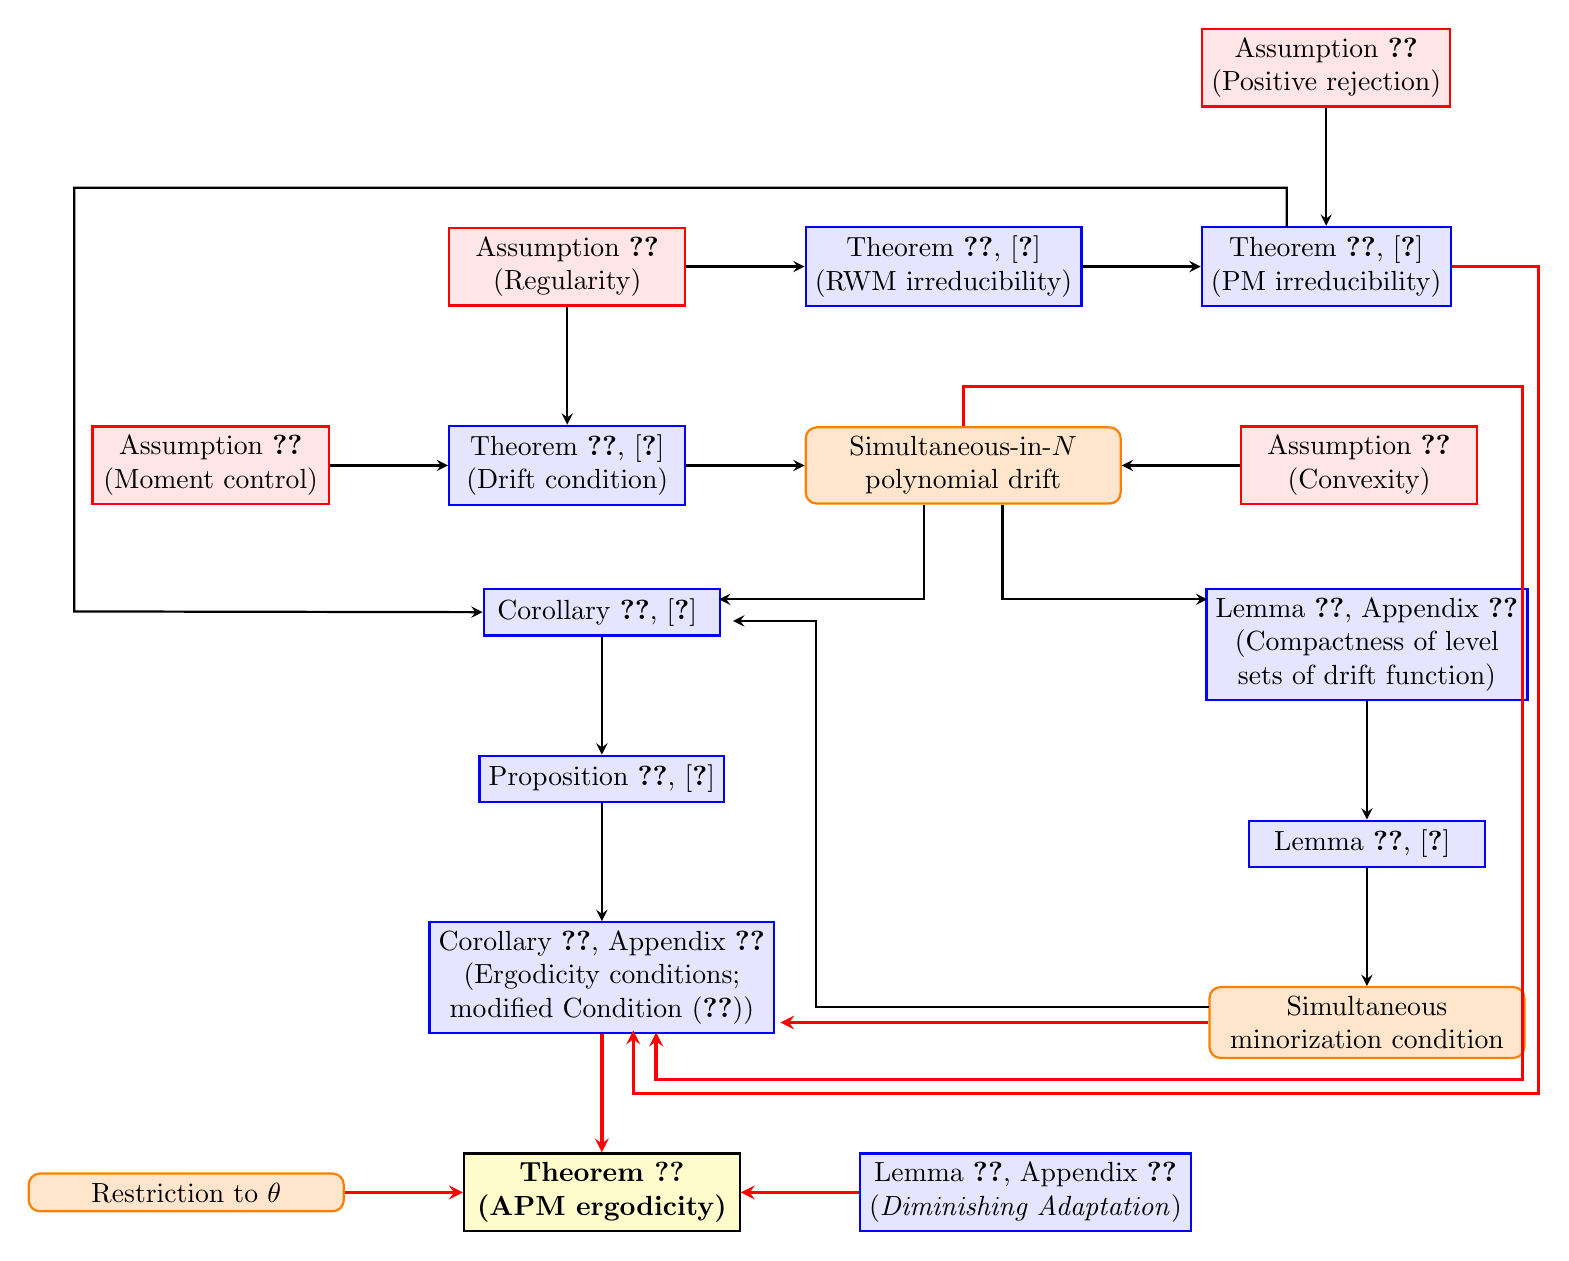
\begin{tikzpicture}[
    node distance=1.5cm,
    assumption/.style={rectangle, draw=red, fill=red!10, thick, minimum width=3cm, align=center},
    theorem/.style={rectangle, draw=blue, fill=blue!10, thick, minimum width=3cm, align=center},
    maintheorem/.style={rectangle, draw=black, fill=yellow!20, thick, minimum width=3.5cm, align=center, font=\bfseries},
    driftbox/.style={rectangle, draw=orange, fill=orange!20, thick, rounded corners, minimum width=4cm, align=center},
    arrow/.style={->, >=stealth, thick},
    highlightarrow/.style={->, >=stealth, thick, draw=red, line width=1.2pt}
]

\node (hyp1) [assumption] {Assumption~\ref{hyp1} \\ (Regularity)};
\node (appthm1) [theorem, right=of hyp1] {Theorem~\ref{appendix:thm1}, \cite{jarner_geometric_2000} \\ (RWM irreducibility)};
\node (appthm2) [theorem, right= of appthm1] {Theorem~\ref{appendix:thm2}, \cite{andrieu_pseudo-marginal_2009} \\ (PM irreducibility)};
\node (hyp4) [assumption, above=of appthm2] {Assumption~\ref{hyp4} \\ (Positive rejection)};

\node (appthm3) [theorem, below=of hyp1] {Theorem~\ref{appendix:thm3}, \cite{andrieu_convergence_2015}\\ (Drift condition)};
\node (hyp3) [assumption, left=of appthm3] {Assumption~\ref{hyp3} \\ (Moment control)};
\node (drift) [driftbox, right=of appthm3] {Simultaneous-in-$N$ \\ polynomial drift};
\node (hyp2) [assumption, right=of drift] {Assumption~\ref{hyp2} \\ (Convexity)};

\node (cor1) [theorem, below left=of drift] {Corollary~\ref{appendix:Corollary1}, \cite{atchade_limit_2010} };
\node (p1) [theorem, below=of cor1] {Proposition~\ref{appendix:proposition1}, \cite{atchade_limit_2010}};
\node (modcor2) [theorem, below=of p1] {Corollary~\ref{appendix:Corollary2bis}, Appendix~\ref{appendixA} \\ (Ergodicity conditions; \\modified Condition~\eqref{appendix:ii})};

\node (thm1) [maintheorem, below=of modcor2] {Theorem~\ref{thm1} \\ (APM ergodicity)};
\node (rest) [driftbox, left=of thm1] {Restriction to $\theta$};
\node (DA) [theorem, right=of thm1] {Lemma~\ref{lemma1}, Appendix~\ref{appendixB}\\ (\textit{Diminishing Adaptation})};


\node (lemma2) [theorem, below right=of drift] {Lemma~\ref{lemma2}, Appendix~\ref{appendixC} \\ (Compactness of level\\ sets of drift function)};
\node (lemma1) [theorem, below=of lemma2] {Lemma~\ref{appendix:lemma1}, \cite{atchade_limit_2010} };
\node (minor) [driftbox, below=of lemma1] {Simultaneous \\ minorization condition};


\draw [arrow] (hyp1) -- (appthm1);
\draw [arrow] (appthm1) -- (appthm2);
\draw [arrow] (hyp4) -- (appthm2);
\draw [highlightarrow] (appthm2) -- ++(1.6,0) -| ++(1.1,0) |- ++(-11.5,-10.5) -- ++(0,0.8)(modcor2);

\draw [arrow] (hyp1)  -- (appthm3); 
\draw [arrow] (hyp3) -- (appthm3); 
\draw [arrow] (hyp2) -- (drift); 
\draw [arrow] (appthm3) -- (drift); 
\draw [highlightarrow] (drift) -- ++(0,1) -| ++(7.1,-8.8) -|++(-11,0.6)  (modcor2); 
\draw [highlightarrow] (minor) --++ (-7.45,0) (modcor2); 

\draw [arrow] (lemma1) -- (minor);
\draw [arrow] (lemma2) -- (lemma1); 

\draw [arrow] (p1) -- (modcor2);
\draw [arrow] (cor1) -- (p1);

\draw [arrow] (drift) ++(-0.5,-0.5) |- ++(-2.6,-1.2)(cor1);
\draw [arrow] (minor) ++(-2,0.2) -- ++ (-5,0) --++(0,4.9) --++(-1.05,0)(cor1);
\draw [arrow] (appthm2) ++ (-0.5,0.5) |- ++(-15.4,0.5) -| ++(0,-5.38) --++ (cor1);

\draw [arrow] (drift) ++(0.5,-0.5) |- ++(2.6,-1.2) (lemma2);

\draw [highlightarrow] (modcor2) -- (thm1); 
\draw [highlightarrow] (rest) -- (thm1); 
\draw [highlightarrow] (DA) -- (thm1);
\end{tikzpicture}
}
\caption{Diagram of the proof of Theorem~\ref{thm1}.
}
\label{diagram}
\end{figure}

\begin{proof}[Proof of Theorem~{\upshape\ref{thm1}}]
First, we prove that the PM algorithm is $\phi$-irreducible and aperiodic. For $N\geq N_0$, under Assumption~\ref{hyp1}, Theorem~\ref{appendix:thm1} establishes that the marginal RWM algorithm associated with the PM algorithm is $\mu_{\text{Leb}}$-irreducible and aperiodic. Building upon this, Assumption~\ref{hyp4} (positive rejection probability) allows us to invoke Theorem~\ref{appendix:thm2}, which confirms that the PM kernel $P_N$ is also $\mu_{\text{Leb}}$-irreducible and aperiodic for all $N$. 

Next, we construct an appropriate function to guarantee that the polynomial drift condition~\eqref{polynomialdrift} in Definition~\ref{def5} holds simultaneously for $P_N$ across all $N \geq N_0$. From Assumption~\ref{hyp2} and the convexity of the function $w \mapsto w^{-\alpha_{0}} \vee w^{\beta_{0}}$ for $w \in \mathcal{W}$, Definition~\ref{def1} implies that for $N \ge N_0$,
\[
\E[W_N^{-\alpha_{0}} \vee W_N^{\beta_{0}}|\theta]  \leq \E[W_{N_0}^{-\alpha_{0}} \vee W_{N_0}^{\beta_{0}}|\theta].
\]
Consequently, taking the essential supremum over $\theta$ gives,
\[
\underset{\theta \in \Theta}{\mathrm{ess\,sup}}\,  \E[W_N^{-\alpha_{0}} \vee W_N^{\beta_{0}}|\theta]  \leq \underset{\theta \in \Theta}{\mathrm{ess\,sup}}\,  \E[W_{N_0}^{-\alpha_{0}} \vee W_{N_0}^{\beta_{0}}|\theta].
\]
From Assumption~\ref{hyp3}, we have $M_{W_{N_0}}=  {\mathrm{ess\,sup} }_{\theta \in \Theta}\, \E[W_{N_0}^{-\alpha_{0}} \vee W_{N_0}^{\beta_{0}}|\theta] <  \infty$.
Therefore, we can conclude that $M_{W_N} = {\mathrm{ess\,sup} }_{\theta \in \Theta}\,  \E[W_N^{-\alpha_{0}} \vee W_N^{\beta_{0}}|\theta]  < \infty$. This directly satisfies Condition~\eqref{appendix:moments} of Theorem~\ref{appendix:thm3} with $\alpha'=\alpha_{0}$ and $\beta'=\beta_{0}$. We now define the function $V : \Theta \times \mathcal{W} \to [1, \infty)$ as
\[
V(\theta, w) = c_\pi^{\eta}\pi^{-\eta}(\theta) (w^{-\alpha} \vee w^{\beta}),
\]
where $c_\pi ={\sup}_{\vartheta \in \Theta} \pi(\vartheta)$, and the parameters are chosen as $\eta = \min(\alpha_{0},1,\beta_{0}-1)/2 \in (0, \min(\alpha_{0},1,\beta_{0}-1))$, $\alpha = (\alpha_{0}+\eta)/2 \in (\eta, \alpha_{0}]$, and $\beta = (\beta_{0}-\eta+1)/2 \in (1, \beta_{0}-\eta)$. With this function and along with Assumption~\ref{hyp1}, we apply Theorem~\ref{appendix:thm3} and we conclude that there exist constants $\bar{w} \in [1, \infty)$, $M \in [1, \infty)$, $c \geq 1$, $\underline{w} \in (0,1]$, and $\delta>0$ such that the polynomial drift condition holds simultaneously for $N \geq N_0$:
\begin{align}
    P_N V(\theta, w) \leq V(\theta, w) - \delta V^{\frac{\beta-1}{\beta}}(\theta, w) + c\ind_\mathcal{C}(\theta, w),
    \label{polydrift}
\end{align}
where $\mathcal{C} =\{(\theta, w) : |\theta|\leq M, w\in [\underline{w}, \bar{w}]\}$. 


To establish the ergodicity of the APM, it remains to verify that the minorization condition~\eqref{appendix:minorization} (see Definition~\ref{def5}) holds for all level sets of the function $V$. In Lemma~\ref{lemma2} in Appendix~\ref{appendixC}, we show that for any $b>1$, the level set 
\(B = \{(\theta, w) \in \Theta \times \mathcal{W} | V(\theta, w) \leq b\} \) of $V$
is compact and has positive Lebesgue measure.

Along with Lemma~\ref{appendix:lemma1} we conclude that there exist $\epsilon_B > 0$ and a probability measure $\nu_B$ such that for all $N \geq N_0$ and for all $B$ level sets of $V$,
\begin{align}
P_N(\theta, w; \cdot) \geq \epsilon_B \ind_B(\theta, w) \nu_B(\cdot).
    \label{minorization}
\end{align}

We have established $\phi$-irreducibility and aperiodicity, together with the existence of polynomial drift and minorization conditions, simultaneously in $N$, over all level sets of the function $V$. Consequently, all assumptions of Corollary~\ref{appendix:Corollary1} are satisfied. Therefore, there exists a level set \( B \subset \Theta \times \mathcal{W} \) of $V$, constants \( \varepsilon_B, c_B > 0 \), and a probability measure \( \nu_B \) such that
\begin{align*}
P_N(\theta,w ;\cdot) &\geq \ind_B(\theta,w)\, \varepsilon_B \nu_B(\cdot), \quad
P_N V(\theta,w) \leq V(\theta,w) - c_B V^{1-\alpha}(\theta,w) + b\, \ind_B(\theta,w),
\end{align*}
with $\sup_B V < \infty$, $\nu_B(B) > 0$, and $c_B \inf_{B^c} V^{1-\alpha} \geq b$.

By Proposition~\ref{appendix:proposition1}, there exists a constant $C$ depending on $\sup_B V$, $\nu(B)$, and $\varepsilon, \alpha, b, c$, such that for any $0 \leq \beta \leq 1 - \alpha$ and $1 \leq \kappa \leq \alpha^{-1}(1 - \beta)$,
\begin{equation*}
(n+1)^{\kappa-1}\,\|P_N^n(\theta,w ; \cdot) - \bar\pi_N(\cdot)\|_{V^\beta} \leq C\,V^{\beta+\alpha\kappa}(\theta,w).
\end{equation*}
Choosing $\beta=0$ and $\alpha=1/\kappa$, and taking the supremum over $N \geq N_0$ and then over $(\theta,w)$, we obtain
\begin{equation}
\lim_{\ell \to \infty} \,
\sup_{(\theta,w) \in \Theta \times \mathcal{W}}
V^{-1}(\theta,w)
\sup_{N \in \mathbb{N}}
\| P^\ell_N((\theta,w), \cdot) - \bar\pi_N \|  = 0,
\label{a1ii}
\end{equation}
which is a generalized version of Condition~\eqref{appendix:ii} in Theorem~\ref{appendix:thm4}.

The remaining two conditions, \eqref{appendix:i} and \eqref{appendix:iii}, required by Theorem~\ref{appendix:thm4} to ensure ergodicity of adaptive MCMC algorithms, follow directly from Corollary~\ref{appendix:Corollary2}. Indeed, the proof in Subsection~4.3 of \cite{atchade_limit_2010} applies to these two points. This yields Corollary~\ref{appendix:Corollary2bis}, which is identical to Corollary~\ref{appendix:Corollary2} except that Condition~\eqref{appendix:ii} is replaced by its generalized form in~\eqref{a1ii}.

Finally, our main result follows directly from the \textit{diminishing adaptation} property of the APM algorithm (Lemma~\ref{lemma1}), together with Corollary~\ref{appendix:Corollary2bis} and the restriction of the function $f$ in Theorem~\ref{appendix:thm4} to $\Theta$. To establish ergodicity of the APM under the generalized Condition~\eqref{a1ii}, we apply exactly the same proof as in Theorem~\ref{appendix:thm4} (see Subsection~4.3.2 of \cite{atchade_limit_2010}), with the sole modification that $f$ is defined only on $\Theta$. This completes the proof of ergodicity for the APM algorithm.
\end{proof}

\section{Synthetic Data Example}
\label{sec:syntheticex}
In this section, a synthetic data example is considered to illustrate the practical verification of Assumptions~\ref{hyp1}--\ref{hyp4}, which are required by Theorem~\ref{thm1}. The APM algorithm (Algorithm~\ref{algo:apm}) is applied to this example, and its performance is subsequently compared with that of the non adaptive method introduced in Section~\ref{sec:review}.

The example involves a Bayesian latent variable model in which the observations \( Y_t |U_t \sim \mathcal{N}(U_t, 1) \), for \( t \in \{1, \ldots, T\} \), are assumed to be conditionally independent given the latent variables \( U_t \). The latent variables are themselves modeled as conditionally independent given a parameter \( \theta \in \mathbb{R} \), with \( U_t |\theta \sim \mathcal{N}\left(\theta, {1}/\{\theta^2 + 1\}\right) \) for each \( t \). A uninformative Gaussian prior \( \theta \sim \mathcal{N}(0, \sigma_0^2) \) is assigned to the parameter, where \( \sigma_0 = 10^5 \). 

This hierarchical model yields the following observed likelihood:
\begin{align*}
    p(y |\theta)
    &= \prod_{t=1}^{T} \varphi\left(y_t ; \theta, \tfrac{\theta^2 + 2}{\theta^2 + 1}\right).
\end{align*}

Although the likelihood is available in closed form, an unbiased positive estimator, constructed using a Monte Carlo method, is employed to align with the context of the PM and APM algorithms. This estimator is defined as
\begin{align}
    \widehat{p}_{T,N}(y |\theta, U) = \prod_{t=1}^{T} \widehat{p}_{N}(y_t |\theta, U_t) = \prod_{t=1}^{T} \frac{1}{N} \sum_{n=1}^{N} \varphi(y_t ; U_{t,n}, 1),
    \label{se:estimator}
\end{align}
where \( U_{t,n} |\theta \sim \mathcal{N}(\theta, 1/\{\theta^2 + 1\}) \) are independent and identically distributed for \( t \in \{1,\ldots, T\} \) and \( n \in \{1,\ldots, N\} \).

The corresponding posterior distribution satisfies
\begin{align}
    \pi(\theta) 
    &\propto \left( \frac{\theta^2 + 1}{\theta^2 + 2} \right)^{\frac{T}{2}} \exp\left\{ -\frac{1}{2} \left( \frac{\theta^2 + 1}{\theta^2 + 2} \sum_{t=1}^{T}(\theta - y_t)^2 + \frac{\theta^2}{\sigma_0^2} \right) \right\}.
    \label{SEpi}
\end{align}
Since the posterior density \( \pi \) is known up to a normalizing constant, a MH algorithm can be implemented. The posterior averages estimates obtained via the MH algorithm are compared to those produced by the PM and APM algorithms, for validation purposes.

In the experimental setup, the data were generated under the parameter value \( \bar\theta = 0 \), with a total of \( T = 200 \) observations. For the implementation of the MH, the PM in Step~\ref{step1} and the APM, the following Gaussian proposal distribution is adopted:
\begin{align}
    q(\vartheta |\theta) = \varphi\left(\vartheta; \theta, l_\textopt^2\frac{2}{T}\right) = \varphi\left(\vartheta; \theta, \frac{8}{T}\right),
    \label{intru}
\end{align}
where the scaling \( l_\text{opt}^2 = 4 \) follows the recommendation of \cite{schmon_large-sample_2021} for the case of a one-dimensional parameter, and the term \( 2/T \) corresponds to the inverse of the Fisher information evaluated at \( \bar{\theta} = 0 \), which is the parameter value used to generate the synthetic data (see Theorem 10.1 in \cite{Vaart_1998} for a theoretical justification of using the inverse Fisher information matrix as the proposal variance).

The explicit verification of Assumptions~\ref{hyp1}--\ref{hyp4} implies that Theorem~\ref{thm1} can be applied to this synthetic data example, thereby ensuring that the APM algorithm is ergodic.
\begin{proposition}
\label{se:verification}
Assumptions~\ref{hyp1}--\ref{hyp4} hold for the synthetic data example.
\end{proposition}
\begin{proof}[Proof of Proposition~\ref{se:verification}]
See Appendix~\ref{appendixD0}.
\end{proof}

In the following, a numerical comparison is carried out between the APM algorithm and its non adaptive counterpart described in Section~\ref{sec:review}.

To ensure a fair and reproducible comparison, the APM and the non adaptive methods were implemented using consistent coding practices, with shared components reused when applicable. Simulations were conducted in the same computational environment (Linux kernel 5.14, AMD Ryzen 9 5950X, 62~GB RAM) using \texttt{R} version 4.2.1, random seeds were fixed to ensure reproducibility, and execution times were recorded via \texttt{Sys.time}.

Key parameters were aligned across both implementations to support a meaningful comparison. Both methods used an initial number of particles \( N_0 = N_1 = 100 \), a common starting point \( \theta_0 = 0 \), the same step size \( a = a_1 = 1 \). The APM algorithm (Algorithm~\ref{algo:apm}) was run for \(10^6\) iterations, matching iterations used in Step~\ref{step3} of the non adaptive method. The same burn-in of $2 \cdot 10^5$ (20\% of total samples) was considered for the APM algorithm and for the final run (Step~\ref{step3}) of the non adaptive method. The burn-in was determined through Geweke diagnostics (see \cite{geweke_1995})  when comparing the first 20\% versus last 50\% of chains. Table~\ref{tab:method_comparison} in Appendix~\ref{appendixD2} summarizes the corresponding settings.

Quantitative comparison between the methods was based on posterior mean and variance estimates, averaged over 10 independent runs. For each run, we also evaluated the acceptance rate \( \widehat{P} \) and the estimate \( \widehat{IF} \) of the inefficiency factor (see Equation~\eqref{inefficiency}) computed using the \textit{overlapping batch means} method of~\cite{flegal_batch_2010}. These metrics, along with execution times, were systematically compared across both methods. Visual comparisons were also performed using trace and autocorrelation plots of the parameter \( \theta \), allowing qualitative assessment of sampling efficiency and mixing behavior (see Appendix~\ref{appendixD4}).

Prior to detailing the implementation of the non adaptive method, we present benchmark results obtained using the MH algorithm on the same synthetic example. This serves as a validation of the posterior estimates produced by the non adaptive method. The MH algorithm was executed 10 times, each with \(10^6\) iterations and using the proposal distribution defined in Equation~\eqref{intru}. The resulting posterior mean was \( \hat\theta_\text{MH} = -0.026 \pm 0.0002 \), and the posterior variance was \( \hat\sigma^2_\text{MH} = 0.009 \pm 0.0000 \). We now detail the implementation steps for the non adaptive method (Section~\ref{sec:review}) on the synthetic example.

First and for each run, a preliminary execution of the PM algorithm was conducted using \( N_1 = 100 \) particles and the proposal variance specified in Equation~\eqref{intru}. Summary results of all runs are reported in Table~\ref{se:tab1}.
    \begin{table}[h]
    \centering
    \caption{Preliminary run of the PM algorithm on the synthetic example with \(10^5\) iterations and \(N_1 = 100\). Reported values are means and standard deviations over 10 independent runs.}
    \begin{tabular}{l@{\hspace{3cm}}c}
    \hline
    Statistic & Mean $\pm$ SD \\
    \hline
    Posterior Mean $\hat\theta_{100}$ & $-0.025 \pm 0.0021$ \\
    Posterior Variance $\widehat{\sigma}_{100}^2$ & $0.009 \pm 0.0002$ \\
    Acceptance Rate $\widehat P$ (\%) & $15.881 \pm 0.4559$ \\
    \hline
    \end{tabular}
    \label{se:tab1}
    \end{table}

 Recall that in this example the parameter dimension is \( d = 1 \), and the value \( \sigma_{\text{opt}} = 1.16 \) was chosen from Table 1 in \cite{schmon_large-sample_2021} for implementing Step~\ref{step2}. For each run, using the estimate \( \hat\theta_{100} \), the standard deviations \( \sigma_N(\hat \theta_{100}) \) of the additive noise \( \omega_N(\hat \theta_{100}) \) were estimated for various values of \( N \), following the approach in Step~\ref{step2}. These estimates were obtained via Monte Carlo simulation using the identity in Equation~\eqref{estimationsd} and $10^4$ iterations for each $N$, with the goal of identifying an optimal number of particles \( N_{\text{opt}} \) such that \( \hat \sigma_{N_{\text{opt}}}(\hat \theta_{100}) \approx 1.16 \).
    \label{dichotomic}
    The \textit{dichotomic search} interval was initialized as \( [100, 1000] \) for the number of particles. At each iteration, the estimate \( \hat\sigma_N(\hat\theta_{100}) \) was computed at the current midpoint of the interval. Initially, evaluations were performed at \( N = 100 \) and \( N = 1000 \). The midpoint value \( N = 550 \) was then tested. If the estimated standard deviation at the midpoint exceeded the target value \( \sigma_{\mathrm{opt}} = 1.16 \), the lower bound of the interval was updated to the midpoint; otherwise, the upper bound was updated accordingly. This bisection procedure was repeated until the length of the final interval reached \( a_1 = 1 \). An example run of this \textit{dichotomic search} is detailed in Appendix~\ref{appendixD1}.

\begin{table}[h]
\centering
\caption{Optimal $N$ for multiple independent runs.}
\label{tab:optimal_N_runs}
\begin{tabular}{@{}l *{10}{c} @{}}

\toprule
 {Run} & 1 & 2 & 3 & 4 & 5 & 6 & 7 & 8 & 9 & 10 \\
\hline
{Optimal} ${N}$ & 203 & 202 & 199 & 201 & 208 & 201 & 202 & 204 & 199 & 201 \\
$\hat{\sigma}_{N}{(\hat\theta_{100})}$ & 1.162 & 1.161 & 1.158 & 1.156 & 1.160 & 1.162 & 1.161 & 1.160 & 1.157 & 1.160 \\
\bottomrule
\end{tabular}
\end{table}

Table~\ref{tab:optimal_N_runs} summarizes the results of the optimal \( N \) for each of the 10 independent runs. In all cases, the optimal number of particles was found within the range \( \{199, \ldots, 208\} \). Detailed values of \( N \) selected by the \textit{dichotomic search} algorithm, along with the corresponding estimates of \( \sigma_N(\hat\theta_{100}) \), are provided in Table~\ref{comp:step2} in Appendix~\ref{appendixD3}.

Finally, the PM algorithm was executed for each run using the corresponding optimal number of particles \( N_{\text{opt}} \) identified earlier. The Markov chain was initialized at \( \hat{\theta}_{100} \), and a Gaussian random walk proposal with variance \( 4 \hat{\sigma}_{100}^2 \) was used, where \( \hat{\sigma}_{100} \) is the posterior standard deviation estimate from Step~\ref{step1}. Posterior estimates, averaged over 10 independent runs and reported in the first column of Table~\ref{se:tab3}, closely match those obtained using the MH algorithm, confirming the correctness of the implementation. 

In the remainder of this section, we demonstrate how the APM outperforms the non adaptive method, in the context of this synthetic data example. The APM algorithm can be run directly, thereby eliminating the need for the preliminary tuning steps. Furthermore, we show that, for the example under study, the APM algorithm achieves superior performance in terms of execution time compared to its non adaptive counterpart.

Additional APM specific parameters were set as follows: the \textit{epoch} size was \( K = 100 \), the adaptation tolerance was \( \sigma_\text{e} = 0.015 \) and the adaptation probability was defined as \( p_j = 1/\sqrt{j} \), a standard choice in adaptive MCMC schemes~\cite{roberts_examples_2009}.

As outlined in Section~\ref{sec:APM}, a transformation of the proposed auxiliary variables \( V \) was applied to estimate the likelihood at a fixed parameter value \( \hat{\theta}_\ell \). For each \textit{epoch} \( j \), with \( \ell = Kj \), the auxiliary variables \( V_{i,t,n}|\vartheta_i \sim \mathcal{N}(\vartheta_i, 1/\{\vartheta_i^2 + 1\}) \) for \( i \in \{\ell - K + 1, \ldots, \ell\} \), \( t \in \{1, \ldots, T\} \), and \( n \in \{1, \ldots, N_{i-1}\} \), were transformed as

\[
\widehat{V}_{i,t,n} = h(V_{i,t,n},\vartheta_i,\hat{\theta}_{i-1}) = \sqrt{\frac{\vartheta_i^2 + 1}{\hat{\theta}_{i-1}^2 + 1}}(V_{i,t,n} - \vartheta_i) + \hat{\theta}_{i-1},
\]
so that \( \widehat{V}_{i,t,n}|\hat{\theta}_{i-1} \sim \mathcal{N}(\hat{\theta}_{i-1}, 1/\{\hat{\theta}_{i-1}^2 + 1\}) \). This transformation allowed the evaluation of the log-likelihood estimator at $\hat\theta_{i-1}$ and $\widehat{V}_i=\{\widehat{V}_{i,t,n}\}_{1 \leq t\leq T, 1 \leq n\leq N_{i-1}}$. Using Equation~\eqref{se:estimator} we get,
\begin{align*}
   \log\{ \widehat{p}_{T, N_{i-1}}(y |\hat{\theta}_{i-1}, \widehat{V}_i) \} = \sum_{t=1}^{T} \log \left\{\frac{1}{N_{i-1}} \sum_{n=1}^{N_{i-1}} \varphi(y_t ; \widehat{V}_{i,t,n}, 1) \right\}.
\end{align*}
 The standard deviation of this log-likelihood is then computed after each \textit{epoch} using Equation~\eqref{hatsigma}.

\begin{table}[h]
\caption{Comparison of summary statistics and execution times, with the same initial values for both approaches, between the PM and the APM algorithms using $10^6$ iterations ($20\%$ Burn-in) across 10 runs. MH results with a 20\% Burn-in are used as the ground truth. Values are reported as mean $\pm$ standard deviation except for $N$ using median [min,max].}
\centering
\begin{tabular}{lccc}
\hline
 & MH & Non adaptive & Adaptive \\
\hline
Optimal N & – & 202 [199,208] & 199 [196,202] \\
Posterior Mean & $-0.0260 \pm 0.0002$ & $-0.0260 \pm 0.0004$ & $-0.0260 \pm 0.0005$ \\
Posterior Variance & $0.00909 \pm 0.00003$ & $0.00909 \pm 0.00003$ & $0.00910 \pm 0.00004$ \\
Acceptance Rate $\widehat{P}$ (\%) & $48.66 \pm 0.04$ & $26.14 \pm 0.20$ & $25.04 \pm 0.15$ \\
Inefficiency Factor $\widehat{IF}$ & $4.45 \pm 0.06$ & $11.77 \pm 0.24$ & $12.37 \pm 0.49$ \\
Execution Time & – & 1h19m31s $\pm$ 11m21s & \textbf{1h02m22s $\pm$ 1m03s} \\
\hline
\end{tabular}
\label{se:tab3}
\end{table}

\begin{figure}
    \centering
    \includegraphics[width=0.9\linewidth]{Trace_N.pdf}
    \caption{Trace of \( N \) using \( 10^4 \) epochs of $100$ iterations across 10 APM runs.}
    \label{se:fig2}
\end{figure}

As shown in the second column of Table~\ref{se:tab3}, the posterior mean and variance are estimated as \( \hat{\theta} = -0.026 \) and \( \hat{\sigma}^2 = 0.009 \), respectively. These estimates coincide with those obtained in Step~\ref{step3} of the non adaptive procedure and with the MH algorithm. The inefficiency factor is \(\widehat{IF} = 12.372\), slightly higher than in the non adaptive case, though the difference is minor. This increase is expected, as the inefficiency factor decreases with larger values of \(N\). The APM algorithm begins with \(N_0 = 100\), increasing \(N\) gradually during adaptation.  
Although a 20\% burn-in period removes the very first iterations from the analysis, part of the adaptation phase remains, which may slightly reduce efficiency compared to the non adaptive procedure. In contrast, Step~\ref{step3} uses the optimal number of particles, \( N_\text{opt} \in \{199, \ldots, 208\} \), allowing for greater efficiency from the outset. Starting the APM with \(N\) near \(N_\text{opt}\) would likely yield more similar performance.

From a computational perspective, however, it is generally advantageous not to use \(N_\text{opt}\) from the start. Instead, beginning with a smaller value while the algorithm is still in its warm-up phase, and increasing it progressively as needed, is more efficient. This is precisely the strategy of the APM algorithm, which achieves substantial time savings without loss of accuracy.

Over 10 runs, the APM algorithm required an average of 1 hour, 2 minutes, and 22 seconds, compared with 1 hour, 19 minutes, and 31 seconds for the full non adaptive method. Thus, the APM is approximately \(1.275\) times faster, providing improved computational efficiency while maintaining accuracy in the posterior estimates. Moreover, when accounting for execution time, the APM delivers \(21\%\) more effective samples per minute (1037 vs.~855), despite a slightly higher inefficiency factor. The latter is computed as
\[
\frac{\text{Sample size}}{\widehat{{IF}} \times \text{Time (min)}} 
\;\overset{\text{APM}}{=}\; 
\frac{800 \, 000}{12.372 \times 62.37} 
= 1\,037 
\quad \text{effective samples/minute}.
\]

Figure~\ref{se:fig2} shows the evolution of the number of particles \( N \) during each APM run. In all cases, \( N \) gradually stabilizes near the corresponding optimal value, indicating effective adaptation. The median of the optimal values \( N_{\text{opt}} \), defined as the final number of particles used in each run, ranged from 196 to 202 across the 10 APM runs. This range is consistent with that obtained using the non adaptive method, and although slightly narrower, the difference is minimal. This suggests that both approaches identify similar values for \( N \), with no significant practical difference, supporting the fairness of the comparison and the robustness of the tuning strategy.

A slightly narrower interval for \( N_{\text{opt}} \) in the non adaptive method could have been obtained by increasing the number of Monte Carlo iterations in Step~\ref{step2} from \( 10^4 \) to \( 10^5 \), at the cost of roughly one additional hour of computation. Under such settings, our experiments indicate that the APM algorithm would be approximately 2.2 times faster than its non adaptive counterpart.

Additional convergence diagnostics, including autocorrelation and trace plots of \( \theta \), are provided in Appendix~\ref{appendixD4}.

\section{Real Data Study}
\label{sec:realex}
In this section, we evaluate the performance of the APM algorithm relative to the non adaptive method using a real dataset from a longitudinal cohort study of preschool-aged children in Indonesia. The dataset was previously analyzed by \cite{zeger_generalized_1991} via Bayesian mixed-effects models, and later by \cite{schmon_large-sample_2021} to illustrate weak convergence properties of PM chains. We use the same modeling framework as in~\cite{schmon_large-sample_2021}.

The data consist of \(1200 \) repeated binary responses observed across \( T = 275 \) subjects. Each response indicates the presence or absence of a respiratory infection. Covariates include age, sex, height, a vitamin deficiency indicator, a below-average height indicator, two seasonal terms, and an intercept, yielding a total of eight covariates.

To account for intra-subject correlation, a subject-specific random intercept \( U_t|\tau \sim \mathcal{N}(0, \tau) \) is introduced for each \( t \in \{1, \dots, T\} \), with \( \tau > 0 \). Conditional on \( \theta = (\beta, \tau) \in \mathbb{R}^9 \), the variables \( U_t \) are mutually independent.

Let \( Y_t = (Y_{t,1}, \dots, Y_{t,J_t}) \in \{0,1\}^{J_t} \) denote the binary responses observed for subject \( t \), where \( J_t \) represents the number of repeated measurements for that subject. Conditionally on the random effect \( U_t \in \mathbb{R} \) and parameters \( \theta \), \( Y_t \) are modeled as independent variables via a logistic regression model.
\[
g(y_t | u_t, \theta) = \prod_{j=1}^{J_t} \frac{\exp(y_{t,j} \eta_{t,j})}{1 + \exp(\eta_{t,j})}, \quad \eta_{t,j} = c_{t,j}^\top \beta + u_t,
\]
where \( c_{t,j} \in \mathbb{R}^{8} \) denotes the covariate vector. The random effects density is given by
\[
f(u_t | \theta) = \varphi(u_t; 0, \tau).
\]
The prior on \( \theta \) factorizes as
\[
p(\theta) = p(\beta) p(\tau) = \varphi(\beta; 0_{8}, 10^4 I_{8}) \cdot p(\tau; 1, 1.5),
\]
where \( p(\tau; a_1, a_2) \) denotes the density of an inverse-gamma distribution with shape \( a_1 \) and scale \( a_2 \), i.e.,
\[
p(\tau; a_1, a_2) = \frac{1}{\Gamma(a_1)} \cdot \frac{a_2^{a_1}}{\tau^{a_1 + 1}} \exp\left( -\frac{a_2}{\tau} \right).
\]
This setup yields the following likelihood function,
\[
p_T(y | \theta) = \prod_{t=1}^T \int_{\mathbb{R}} \left[ \prod_{j=1}^{J_t} \frac{\exp(y_{t,j}(c_{t,j}^\top \beta + u))}{1 + \exp(c_{t,j}^\top \beta + u)} \right] \varphi(u; 0, \tau) \, \mathrm{d}u,
\]
The resulting posterior distribution is therefore given by:
\begin{align*}
    \pi(\theta) 
    &\propto p_T(y | \theta) \, p(\theta) \\
    &= \left\{ \prod_{t=1}^T \int_{\mathbb{R}} \prod_{j=1}^{J_t} \frac{\exp \left\{ y_{t,j}(c_{t,j}^\top \beta + x) \right\}}{1+\exp \left\{ c_{t,j}^\top \beta + x \right\}} \varphi(x; 0, \tau) \, \mathrm{d}x \right\} \\
    &\qquad  \varphi(\beta; 0_{8}, 10^4 I_{8}) \, p(\tau; 1, 1.5).
\end{align*}

\begin{remark}
The posterior \( \pi(\theta) \) cannot be evaluated pointwise due to intractable integrals in the likelihood. Hence, direct implementation of the MH algorithm is not feasible.
\end{remark}
\noindent
Within the PM and APM frameworks, the likelihood is estimated using the Classical Importance Sampling. The estimator takes the form
\[
\widehat{p}_{T,N}(y | \theta, U) = \prod_{t=1}^T  \frac{1}{N} \sum_{n=1}^N \varpi(y_t, U_{t,n}, \theta),
\]
where the importance weights are defined by
\[
\varpi(y_t, U_{t,n}, \theta) = \frac{g(y_t | U_{t,n}, \theta) f(U_{t,n} | \theta)}{s(U_{t,n} | y_t, \theta)}, \quad s(U_{t,n} | y_t, \theta) = \varphi(U_{t,n}; \hat{u}_t, \tau),
\]
where \( U_{t,n} \sim \mathcal{N}(\hat{u}_t, \tau) \) and \( \hat{u}_t = \argmax_{u}  g(y_t | u, \theta) f(u | \theta) \).

It can be shown that this likelihood estimator is unbiased and positive. Substituting the expressions for \( g \), \( f \), and \( s \), the estimator becomes
\begin{align}
    \widehat{p}_{T,N}(y | \theta, U) 
= \prod_{t=1}^T \frac{1}{N} \sum_{n=1}^N 
\frac{\left[ \prod_{j=1}^{J_t} \frac{\exp\{y_{t,j}(c_{t,j}^\top \beta + U_{t,n})\}}{1 + \exp\{c_{t,j}^\top \beta + U_{t,n}\}} \right] \varphi(U_{t,n}; 0, \tau)}{\varphi(U_{t,n}; \hat{u}_t, \tau)}.
\label{re:estim}
\end{align}


In this application, it is recalled that the parameter dimension is \( d = 9 \). To implement both the non adaptive and the APM algorithm, the following Gaussian proposal distribution is adopted:
\begin{align}
    q(\vartheta |\theta) = \varphi\left(\vartheta; \theta, \frac{l_\textopt^2}{d}{\Sigma}_p\right) = \varphi\left(\vartheta; \theta, \frac{2.2^2}{9}{\Sigma}_p\right),
    \label{intru2}
\end{align}
where the scaling parameter \( l_{\text{opt}} = 2.2 \) follows the recommendation of \cite{schmon_large-sample_2021}, 
and \( \Sigma_p \) is set to the value used in \cite{schmon_large-sample_2021}. Note that this value is provided only in the accompanying program of article~\cite{schmon_large-sample_2021} and not explicitly stated in the text 
(see Appendix~\ref{appendixE2} for the exact value of \( \Sigma_p \)).

Verifying Assumptions~\ref{hyp1}, \ref{hyp3}, and \ref{hyp4} is nontrivial due to the intractability of the posterior distribution. In contrast, Assumption~\ref{hyp2} holds whenever the likelihood estimator is constructed via Classical Importance Sampling.

The same procedure outlined in Section~\ref{sec:syntheticex} will be followed for the comparison between the non adaptive method and the APM algorithm, and for this reason, some of the explanatory details will be omitted. In this example, simulations were conducted using the same computational environment and practices as described for the synthetic data example in Section~\ref{sec:syntheticex}. Similarly, key parameters were aligned across both implementations. The APM algorithm (Algorithm~\ref{algo:apm}) was run for \(10^6\) iterations with burn-in of $40\%$, matching iterations (with same burn-in) used in Step~\ref{step3} of the non adaptive method. Both methods used an initial number of particles \( N_0 = N_1 = 10 \), a common starting point \( \theta_0 \), and the same step size \( a = a_1 = 1 \). Table~\ref{tab:method_comparison2} in Appendix~\ref{appendixE2} summarizes the corresponding settings.

As in Section~\ref{sec:syntheticex}, the quantitative comparison between the methods was carried out using posterior mean and variance estimates, averaged over 10 independent runs. In the real data example, since $d = 9$, the Euclidean norm of the posterior estimator was reported. For each run, the acceptance rate $\widehat{P}$, the estimated inefficiency factor $\widehat{\text{IF}}$, and the execution time were recorded. The inefficiency factor was obtained by first estimating it for each component and subsequently summing over all components. Trace and autocorrelation plots for each component of the parameter $\theta$ are presented in Appendix~\ref{appendixE4}.

The implementation steps for the non adaptive method (Section~\ref{sec:review}) on the real data example are now described. First and for each run, a preliminary execution of the PM algorithm was conducted using \( N_1 = 10 \) particles and the proposal distribution specified in Equation~\eqref{intru2}. A summary of the results from all runs is presented in Table~\ref{re:tab1}.
    \begin{table}[h]
    \centering
    \caption{Preliminary run of the PM algorithm on the real data example with \(10^5\) iterations and \(N_1 = 10\). Reported values are the mean and standard deviation of euclidean norms over 10 independent runs.}
    \begin{tabular}{l@{\hspace{3cm}}c}
    \hline
    Statistic & $ \text{Mean}\pm  \text{SD}$ \\
    \hline
    Norm of Posterior Mean $\hat\theta_{10}$ & $3.093 \pm 0.0184$ \\
    Norm of Posterior Covariance $\widehat{\Sigma}_{10}$ & $0.388 \pm 0.0182$ \\
    Acceptance Rate $\widehat P$ (\%) & $7.233 \pm 0.3386$ \\
    \hline
    \end{tabular}
    \label{re:tab1}
    \end{table}

 Recall that in this example the parameter dimension is \( d = 9 \), and the value \( \sigma_{\text{opt}} = 1.44 \) was chosen from Table 1 in \cite{schmon_large-sample_2021} for implementing Step~\ref{step2}. For each run, using the estimate \( \hat\theta_{10} \), the standard deviations \( \sigma_N(\hat \theta_{10}) \) of the additive noise \( \omega_N(\hat \theta_{10}) \) were estimated for various values of \( N \). These estimates were obtained via Monte Carlo using $10^4$ iterations for each $N$. The \textit{dichotomic search} interval was initialized as \( [10, 100] \) for the number of particles and terminated when the length of the final interval reached \( a_1 = 1 \). The results summary are in Table~\ref{tab:optimal_N_sigma2} showing the optimal $N$ of each run and the corresponding $\hat{\sigma}_{N}{(\hat\theta_{10})}$. The optimal number of particles was found within the range \( \{21, 22, 23\} \). Details of the estimations of each run are in Table~\ref{re:step2} in Appendix~\ref{appendixE3}.

\begin{table}[h]
\centering
\caption{Optimal $N$ and corresponding $\hat\sigma_{N_{\text{opt}}}(\hat\theta_{10})$ values for multiple independent runs.}
\label{tab:optimal_N_sigma2}
\begin{tabular}{@{}l *{10}{c} @{}}
\toprule
 {Run} & 1 & 2 & 3 & 4 & 5 & 6 & 7 & 8 & 9 & 10 \\
\hline
{Optimal} ${N}$ & 22 & 22 & 22 & 22 & 22 & 22 & 21 & 21 & 21 & 23 \\
$\hat{\sigma}_{N}{(\hat\theta_{10})}$ & 1.436 & 1.433 & 1.447 & 1.430 & 1.458 & 1.425 & 1.460 & 1.429 & 1.454 & 1.444 \\
\bottomrule
\end{tabular}
\end{table}

Finally, the PM algorithm was executed for each run using the corresponding optimal number of particles \( N_{\text{opt}} \) identified earlier. The Markov chain was initialized at \( \hat{\theta}_{10} \), and a Gaussian random walk proposal with variance \( \{2.2^2/9\} \widehat{\Sigma}_{10} \) was used, where \( \widehat{\Sigma}_{10} \) is the posterior covariance estimate from Step~\ref{step1}. The euclidean norm of posterior estimates is averaged over 10 independent runs and reported in the first column of Table~\ref{re:tab3}. 

In the remainder of this section, we detail the implementation of the APM algorithm on the real data example. Additional APM specific parameters were set as follows: the \textit{epoch} size was \( K = 100 \), the adaptation tolerance was \( \sigma_\text{e} = 0.015 \) and the adaptation probability was defined as \( p_j = 1/\sqrt{j} \).

As outlined in Section~\ref{sec:APM}, a transformation of the proposed auxiliary variables \( V \) was applied to estimate the likelihood at a fixed parameter value \( \hat{\theta}_\ell \). For each \textit{epoch} \( j \), with \( \ell = Kj \), the auxiliary variables of the \textit{epoch} $j$, \( V_{i,t,n}|\vartheta_i \sim \mathcal{N}(\hat {v}_{i,t}, \uptau_{i}) \), where \( i \in \{\ell-K+1, \ldots, \ell\} \), $t \in \{1, \ldots, T\} $, $n \in \{1, \ldots, N_{i-1}\}$, $\hat {v}_{i,t} = \argmax_{u}  g(y_t | u, \vartheta_i) f(u | \vartheta_i)$,  and $\uptau_i$ is the last component of $\vartheta_i$, were transformed as
\[
\widehat{V}_{i,t,n} = h(V_{i,t,n}, \vartheta_i, \hat\theta_{i-1}) = \sqrt{\frac{\hat \tau_{i-1}}{\uptau_{i}}}(V_{i,t,n} - \hat {v}_{i,t}) + \widehat{\hat{u}}_{i-1,t},
\]
where $\widehat{\hat{u}}_{i-1,t}=\argmax_{u}  g(y_t | u, \hat\theta_{i-1}) f(u | \hat\theta_{i-1})$, so that \( h(V_{t,n}) \sim \mathcal{N}\left(\widehat{\hat{u}}_{i-1,t}, \hat \tau_{i-1}\right) \). This enabled the evaluation of the log-likelihood estimator \( \log\{\widehat{p}_{T,N_{i-1}}(y|\hat\theta_{i-1},\widehat{V}_i)\} \) using Equation~\eqref{re:estim}, 
{\small
\begin{align*}
    \log\{\widehat{p}_{T,N_{i-1}}(y|\hat\theta_{i-1},\widehat{V}_i)\}
= \sum_{t=1}^T \log\left\{ \frac{1}{N_{i-1}} \sum_{n=1}^{N_{i-1}} 
\frac{\left[ \prod_{j=1}^{J_t} \frac{\exp\{y_{t,j}(c_{t,j}^\top \hat\beta_{i-1} + \widehat{V}_{i,t,n})\}}{1 + \exp\{c_{t,j}^\top \hat\beta_{i-1} + \widehat{V}_{i,t,n}\}} \right] \varphi(\widehat{V}_{i,t,n}; 0, \hat\tau_{i-1})}{\varphi(\widehat{V}_{i,t,n}; \widehat{\hat{u}}_{i-1,t}, \hat\tau_{i-1})} \right \},
\end{align*}
}
where $\hat\beta_{i-1}$ are the first eight components of $\hat\theta_{i-1}$ and $ \hat\tau_{i-1}$ is the last one. The standard deviation of this log-likelihood estimate was estimated using Equation~\eqref{hatsigma}.
\begin{table}[h]
\caption{Comparison of summary statistics and execution times, with same initial values for both approaches, between the PM and the APM algorithms using $10^6$ iterations (with 40\% burn-in) across 10 runs. Values are reported as mean $\pm$ standard deviation except for $N$ using median[min,max].}
  \centering
  \begin{tabular}{lcc}
    \hline
     & Non adaptive & Adaptive \\
    \hline
    Optimal N & $22[21,23]$ & $22[21,24]$\\
    Norm of Posterior Mean & $3.102 \pm 0.0042$ & $3.103 \pm 0.0033$ \\
    Norm of Posterior Variance & $0.386 \pm 0.0029$ & $0.386 \pm 0.0028$ \\
    Acceptance Rate $\widehat{P}$ (\%) & $14.316 \pm 0.3638$ & $14.156 \pm 0.1733$ \\
    Inefficiency factor $\widehat{IF}$ & $86.891 \pm 3.6771$ & $85.081 \pm 3.9266$ \\
    Execution time & {11h10min51s} $\pm$ 30min37s& {11h07min05s} $\pm$ 33min45s \\
    \hline
  \end{tabular}
  \label{re:tab3}
\end{table}

\begin{figure}
    \centering
    \includegraphics[width=0.9\linewidth]{Trace_N2.pdf}
    \caption{Trace of \( N \) using \( 10^4 \) \textit{epochs} of $100$ iterations across 10 APM runs applied on the real data Example.}
    \label{re:fig2}
\end{figure}

As shown in the second column of Table~\ref{se:tab3}, the Euclidean norms of the posterior means and variances match the estimates from Step~\ref{step3} of the non adaptive method. The inefficiency factor of the non adaptive method was estimated as \( \widehat{IF} = 86.891 \), slightly higher than that of the APM, giving the latter an efficiency advantage in this case.

Both methods exhibit similar computational performance, with average execution times of approximately 11~hours. 
The APM algorithm provides a gain of about 3 minutes compared to the total runtime of all steps in the non adaptive method. Its main advantage, however, lies in relying on a single process rather than multiple ones, thereby avoiding the overhead and 
complexity associated with the non adaptive approach.

Using a 40\% burn-in (i.e., retaining 600\,000 samples), the effective sample size per minute is computed as in Section~\ref{sec:syntheticex}. With this measure, the adaptive method attains a 3.5\% higher sampling efficiency (8.9 vs.\ 8.6 effective samples per minute).

Figure~\ref{se:fig2} shows the evolution of the number of particles \( N \) during each APM run. In all cases, \( N \) gradually approaches the corresponding optimal value, indicating effective adaptation. The median of the optimal values \( N_{\text{opt}} \), defined as the last number of particles reached in each run, ranged from 21 to 24. This range is slightly larger but consistent with that obtained via the non adaptive method.

Additional convergence diagnostics, including autocorrelation and trace plots of \( \theta \), are provided in Appendix~\ref{appendixE4}.

\section{Conclusion}
\label{sec:conclusion}
In this work, we have made three main contributions. 
First, we proposed an adaptive mechanism that overcomes the tuning difficulties commonly encountered in PM algorithms. Second, we established verifiable sufficient conditions ensuring the ergodicity of the resulting adaptive process. Third, we quantitatively illustrated the benefits of our approach through a series of numerical experiments.

Looking ahead, several avenues for future research remain open. An immediate extension would be to investigate central limit theorems (CLTs) for the APM in order to provide a more complete theoretical characterization. 
It is worth noting, however, that most existing CLTs for adaptive chains require stronger conditions. In particular, \cite{atchade_2012} shows that a CLT holds in the polynomial case if the adaptation random variable converges almost surely, which is not guaranteed under the current adaptation mechanism. Therefore, future work could either focus on establishing a CLT for polynomially ergodic adaptive chains under alternative conditions, or on modifying the adaptation scheme to ensure that the standard convergence assumptions are satisfied.  

Furthermore, in the non adaptive method, the proposal variance changes from Step~\ref{step1} to Step~\ref{step3}, whereas in the current APM scheme, the adaptation mechanism uses a single proposal variance, which may limit its flexibility. Future work would be to explore \textit{dual adaptation} schemes, where both the number of particles $N$ and the proposal distributions are adapted simultaneously.

\section*{Acknowledgments}
Special thanks to Radu Craiu (University of Toronto) for his contribution to the subject of this article.

%\bibliography{article.bib}
% [flatten_tex] Not found: article.bbl.tex
\input{article.bbl}

\appendix
\section{Technical Preliminaries}
\label{appendixA}
\begin{definition}[Simultaneous Strong Aperiodic Geometrical Ergodicity]  
A family $\{P_\gamma\}_{\gamma \in \mathcal{Y}}$ of Markov kernels defined on a space state $(\mathcal{X}, \mathcal{B}(\mathcal{X}))$ is \textit{simultaneously strongly aperiodically and geometrically ergodic} if there exist $C \in \mathcal{B}(\mathcal{X})$, $V: \mathcal{X} \to [1,\infty)$, $\delta > 0$, $\lambda < 1$, and $b < \infty$, such that $\sup_C V < \infty$, and

\begin{enumerate}
    \item[(i)] for each $\gamma \in \mathcal{Y}$, there exists a probability measure $\nu_\gamma(\cdot)$ on $C$ with $P_\gamma(x,\cdot) \geq \delta\nu_\gamma(\cdot)$ for all $x \in C$, and
    
    \item[(ii)] $P_\gamma V(x) \leq \lambda V(x) + b \ind_C(x)$ for all $x \in \mathcal{X}$.
\end{enumerate}
\label{def2}
\end{definition}

\begin{definition}[Geometric Ergodicity]  
A $\phi$-irreducible, aperiodic Markov kernel $P$ defined on $(\mathcal{X}, \mathcal{B}(\mathcal{X}))$ with stationary distribution $\pi(\cdot)$ is \textit{geometrically ergodic} if there exist $\rho < 1$, $R<\infty$, and a function $V: \mathcal{X} \to [1,\infty)$ such that, for all $A \in \mathcal{B}(\mathcal{X})$, $n \geq 1$, and $x \in \mathcal{X}$,
\[
\|P^n(x, \cdot) - \pi(\cdot)\|_V \leq RV(x)\rho^n,
\]
where the $V$-norm of a measure $\mu$ is defined as $\|\mu\|_V=\sup_{f, |f|_\infty\leq V}|\mu(f)|$.
\label{def3}
\end{definition}

\begin{definition}[Polynomial Ergodicity]  
A $\phi$-irreducible, aperiodic Markov kernel $P$ defined on $(\mathcal{X}, \mathcal{B}(\mathcal{X}))$ with stationary distribution $\pi(\cdot)$ is \textit{polynomially ergodic} if there exist constants $R$, $0<\alpha \leq 1$, and a function $V: \mathcal{X} \to [1,\infty)$ such that, for any $0 \leq \beta \leq 1 -\alpha$ 
and $1 \leq \kappa \leq \alpha^{-1}(1 - \beta)$,
\[
\|P^n(x,\cdot) - \pi(\cdot)\|_{V^\beta} \leq R V^{\beta + \alpha\kappa}(x)(n+1)^{1-\kappa}.
\]
\label{def4}
\end{definition}

\begin{definition}[Simultaneous Minorization and Polynomial Drift Conditions]
Let $\{P_\gamma\}_{\gamma \in \mathcal{Y}}$ be a family of Markov transition kernels on a measurable space $(\mathcal{X}, \mathcal{B}(\mathcal{X}))$, where each $P_\gamma$ is $\phi$-irreducible, aperiodic, and admits a stationary distribution $\pi$. The family is said to be:
\begin{enumerate}[(i)]
    \item \textit{Simultaneous in $\gamma$ Polynomial Drift:} There exist a measurable set $C \subseteq \mathcal{X}$, a function $V: \mathcal{X} \to [1,\infty)$, a constant $\alpha \in (0, 1)$, and constants $b, c > 0$ such that, for all $\gamma \in \mathcal{Y}$,
    \[
    P_\gamma V(x) \leq V(x) - c V^{1-\alpha}(x) + b \ind_C(x), \quad \forall x \in \mathcal{X}.
    \]
    \label{polynomialdrift}
    
    \item \textit{Simultaneous in $\gamma$ Minorization:} For every level set $B = \{x \in \mathcal{X} : V(x) \leq b\}$ of $V$ (for some $b > 1$), there exist $\varepsilon_B > 0$ and a probability measure $\nu_B$ such that, for all $\gamma \in \mathcal{Y}$,
    \[
    P_\gamma(x, \cdot) \geq \varepsilon_B \ind_B(x)\, \nu_B(\cdot), \quad \forall x \in \mathcal{X}.
    \]
    \label{appendix:minorization}
\end{enumerate}
\label{def5}
\end{definition}

\begin{theorem}[Theorem 2.1, \cite{jarner_geometric_2000}]
The RWM algorithm satisfying Assumption~\ref{hyp1} is $\mu_{\text{Leb}}$-irreducible and aperiodic.
    \label{appendix:thm1}
\end{theorem}

\begin{theorem}[Theorem 1, \cite{andrieu_pseudo-marginal_2009}]
Let $P$ be a $\phi$-irreducible and aperiodic MH chain with invariant distribution $\pi$. Then, for any $N \geq 1$ such that $\rho_N(\theta, w) > 0$ for all $(\theta, w)$ (as defined in Equation~\eqref{varrho_repar}), the PM kernel $P_N$ is also $\phi$-irreducible and aperiodic.
\label{appendix:thm2}
\end{theorem}

\begin{remark}
In Theorem~\ref{appendix:thm2}, the authors assume that the weights are well-defined using the concept of measure domination. This assumption is not required in our setting, as the weights are explicitly defined as $W_N(\theta) = \widehat{p}_{N,T}(y| \theta, U) / p_T(y| \theta)$.
\end{remark}

\begin{theorem}[Theorem 38, \cite{andrieu_convergence_2015}]
Let \( P_N \) denote a PM kernel with distributions \( Q_{N,\theta}(dw) \) satisfying the moment condition
\begin{align}
    M_{W_N} := \underset{\theta \in \Theta}{\mathrm{ess\,sup}} \int (w^{-\alpha'} \vee w^{\beta'})\, Q_{N,\theta}(dw) < \infty,
\label{appendix:moments}
\end{align}
for some constants \( \alpha' > 0 \) and \( \beta' > 1 \). Assume that the marginal algorithm is a RWM with invariant density \( \pi \) and proposal density \( q \) satisfying Assumption~\ref{hyp1}.

Define the function \( V: \Theta \times \mathcal{W} \to [1,\infty) \) as
\[
V(\theta,w) := c_\pi \pi^{-\eta}(\theta)\left(w^{-\alpha} \vee w^{\beta}\right), \quad \text{with} \quad c_\pi := \sup_{\vartheta \in \Theta} \pi(\vartheta),
\]
for constants \( \eta \in (0, \alpha' \wedge 1 \wedge \beta'-1) \), \( \alpha \in (\eta, \alpha'] \), and \( \beta \in (1, \beta' - \eta) \).

Then, there exist constants \( \overline{w}, M, b \in [1, \infty) \), \( \underline{w} \in (0,1] \), and \( \delta_V > 0 \) such that
\[
P_N V(\theta,w) \leq 
\begin{cases}
V(\theta,w) - \delta_V V^{(\beta-1)/\beta}(\theta,w), & \text{if } (\theta,w) \notin C, \\
b, & \text{if } (\theta,w) \in C,
\end{cases}
\]
where the set \( C \subset \Theta \times \mathcal{W} \) is defined by
\[
C := \left\{ (\theta, w) \in \Theta \times \mathcal{W} : |\theta| \leq M, \, w \in [\underline{w}, \overline{w}] \right\}.
\]
\label{appendix:thm3}
\end{theorem}


\begin{lemma}[Lemma 3.2, \cite{atchade_limit_2010}]
Assume that the invariant distribution of $P_\gamma$, $\pi$, is bounded from below and from above on compact sets. Then, if $C$ is a compact subset of $\mathcal{X}$ with $\mu_\text{Leb}(C) > 0$, there exist a probability measure $\nu$ on $\mathcal{X}$, a positive constant $\varepsilon$ and a set $C \in \mathcal{X}$ such that for any $x\in \mathcal{X}$,
\[
P_\gamma(x, \cdot) \geq \varepsilon \ind_C(x)  \nu(\cdot).
\]
\label{appendix:lemma1}
\end{lemma}

\begin{corollary}[Corollary A.2, \cite{atchade_limit_2010}]
Let \( P \) be a \(\phi\)-irreducible and aperiodic Markov kernel on \( (\mathcal{X}, \mathcal{B}(\mathcal{X})) \). Suppose there exist constants \( b, c > 0 \), a measurable set \( C \), an unbounded measurable function \( V \colon \mathcal{X} \to [1, \infty) \), and \( 0 < \alpha \leq 1 \) such that
\[
PV(x) \leq V(x) - c V^{1-\alpha}(x) + b\, \ind_C(x).
\]
If, in addition, all level sets of \( V \) are 1-small, then there exist a level set \( B \subset \mathcal{X} \), constants \( \varepsilon_B, c_B > 0 \), and a probability measure \( \nu_B \) such that
\begin{align*}
P(x,\cdot) &\geq \ind_B(x)\, \varepsilon_B \nu_B(\cdot), \quad
PV(x) \leq V(x) - c_B V^{1-\alpha}(x) + b\, \ind_B(x),
\end{align*}
with $\sup_B V < \infty$, $\nu_B(B) > 0$, and $c_B \inf_{B^c} V^{1-\alpha} \geq b.$
\label{appendix:Corollary1}
\end{corollary}

\begin{proposition}[Proposition A.1, \cite{atchade_limit_2010}]
Let $P$ be a $\phi$-irreducible and aperiodic transition kernel on $(\mathcal{X}, \mathcal{B}(\mathcal{X}))$.
\begin{enumerate}[(i)]
    \item Assume that there exist a probability measure $\nu$ on $\mathcal{X}$, positive constants $\varepsilon, b, c$, a measurable set $\mathcal{C}$, a measurable function $V:\mathcal{X} \to [1,+\infty)$ and $0 < \alpha \leq 1$ such that
    \begin{align}
    P(x,\cdot) &\geq \varepsilon \ind_\mathcal{C}(x)\nu(\cdot), 
    \qquad PV \leq V - cV^{1-\alpha} + b\ind_\mathcal{C}. 
    \end{align}
    Then $P$ possesses an invariant probability measure $\pi$ and $\pi(V^{1-\alpha}) < +\infty$.
    \item Assume, in addition, that $c \inf_{\mathcal{C}^c} V^{1-\alpha} \geq b$, $\sup_\mathcal{C} V < +\infty$ and $\nu(\mathcal{C}) > 0$. Then there exists a constant $C$ depending on $\sup_\mathcal{C} V$, $\nu(\mathcal{C})$ and $\varepsilon, \alpha, b, c$, such that for any $0 \leq \beta \leq 1 - \alpha$ and $1 \leq \kappa \leq \alpha^{-1}(1 - \beta)$,
    \begin{equation}
    (n+1)^{\kappa-1}\|P^n(x,\cdot) - \pi(\cdot)\|_{V^\beta} \leq CV^{\beta+\alpha\kappa}(x). \label{eq:convergence_rate}
    \end{equation}
\end{enumerate}
\label{appendix:proposition1}
\end{proposition}



\begin{theorem}[Theorem 2.1, \cite{atchade_limit_2010}]
    For a set $C$, denote by $\tau_C$ the return time to $C \times \mathcal{Y}$, $\tau_C = \inf\{n \geq 1 : X_n \in C\}$. Assuming the \textit{diminishing adaptation} condition and that there exist a measurable function $V \colon \mathcal{X} \to [1, +\infty)$ and a measurable set $C$ such that
    \begin{enumerate}[(i)]
    \item $\sup_{C \times \mathcal{Y}} \mathbb{E}_{x,\gamma}[r(\tau_C)] < +\infty$ for some non-decreasing function $r \colon \mathbb{N} \to (0, +\infty)$ such that $\sum_{n=1}^\infty 1/r(n) < +\infty$;
    \label{appendix:i}
    \item there exists a probability measure $\pi$ such that
    \begin{align*}
        \lim_{n\to+\infty} \sup_{x\in\mathcal{X}} V^{-1}(x) \sup_{\gamma \in \mathcal{Y}} \|P_\gamma^n(x,\cdot) - \pi\| = 0;
    \end{align*}
    \label{appendix:ii}
    \item $\sup_\gamma P_\gamma V \leq V$ on $C^c$ and $\sup_{C \times \mathcal{Y}} \{P_\gamma V(x) + V(x)\} < +\infty$,
     \label{appendix:iii}
\end{enumerate}

then,
\[
\lim_{n\to+\infty} \sup_{\{f : |f|_\infty \leq 1\}} \left|\mathbb{E}[f(X_n) - \pi(f)]\right| = 0.
\]
\label{appendix:thm4}
\end{theorem}

\begin{corollary}[Corollary 2.2, \cite{atchade_limit_2010}]
Let \( \{P_\gamma\}_{\gamma \in \mathcal{Y}} \) be a family of \(\phi\)-irreducible and aperiodic Markov kernels on \( (\mathcal{X}, \mathcal{B}(\mathcal{X})) \), each with invariant distribution \( \pi \). If the family satisfies the \textit{Simultaneous Minorization and Polynomial Drift Conditions} (see Definition~\ref{def5}), then:
\begin{enumerate}[(i)]
    \item There exists a non-decreasing function \( r \colon \mathbb{N} \to (0, \infty) \), such that \( \sum_{n=1}^\infty 1/r(n) < \infty \) and
    \[
    \sup_{(x,\gamma) \in C \times \mathcal{Y}} \mathbb{E}_{x,\gamma}[r(\tau_C)] < \infty.
    \]
    \item A probability measure \( \pi \) exists such that
    \[
    \lim_{n \to \infty} \sup_{x \in \mathcal{X}} V^{-1}(x) \sup_{\gamma \in \mathcal{Y}} \|P_\gamma^n(x, \cdot) - \pi\| = 0.
    \]
    \item The inequality \( \sup_\gamma P_\gamma V \leq V \) holds on \( C^c \) and \(
    \sup_{(x,\gamma) \in C \times \mathcal{Y}} \left\{ P_\gamma V(x) + V(x) \right\} < \infty. \)
\end{enumerate}
\label{appendix:Corollary2}
\end{corollary}

\begin{corollary}[Modified Corollary 2.2, \cite{atchade_limit_2010}]
Let \( \{P_\gamma\}_{\gamma \in \mathcal{Y}} \) be a family of \(\phi\)-irreducible and aperiodic Markov kernels on \( (\mathcal{X}, \mathcal{B}(\mathcal{X})) \), each with invariant distribution \( \pi_\gamma \). If the family satisfies the \textit{Simultaneous Minorization and Polynomial Drift Conditions} (see Definition~\ref{def5}), then:
\begin{enumerate}[(i)]
    \item There exists a non-decreasing function \( r \colon \mathbb{N} \to (0, \infty) \), such that \( \sum_{n=1}^\infty 1/r(n) < \infty \) and
    \[
    \sup_{(x,\gamma) \in C \times \mathcal{Y}} \mathbb{E}_{x,\gamma}[r(\tau_C)] < \infty.
    \]
    \item A probability measure \( \pi_\gamma \) exists such that
    \[
    \lim_{n \to \infty} \sup_{x \in \mathcal{X}} V^{-1}(x) \sup_{\gamma \in \mathcal{Y}} \|P_\gamma^n(x, \cdot) - \pi_\gamma\| = 0.
    \]
    \item The inequality \( \sup_\gamma P_\gamma V \leq V \) holds on \( C^c \) and \(
    \sup_{(x,\gamma) \in C \times \mathcal{Y}} \left\{ P_\gamma V(x) + V(x) \right\} < \infty. \)
\end{enumerate}
\label{appendix:Corollary2bis}
\end{corollary}

\begin{theorem}[Theorem 7, \cite{andrieu_establishing_2016}]
If there exists a probability space with random variables \( X' \) and \( Y' \) having the same distributions as \( X \) and \( Y\), respectively, and such that
\[\mathbb{E}[Y'|X'] = X' \quad \text{a.s.},\]
then \( X \preceq_{cx} Y \).
    \label{appendix:thm5}
\end{theorem}

\begin{corollary}[Corollary 3.A.22, \cite{shaked_stochastic_2007}]
Let \( X_1 \) and \( X_2 \) be a pair of independent random variables, and let \( Y_1 \) and \( Y_2 \) be another pair of independent random variables. If \( X_i {\preceq_{cx}} Y_i \), for \( i = 1, 2 \), then
\[X_1 X_2 \preceq_{cx} Y_1 Y_2.\]
\label{appendix:corollary3}
\end{corollary}

\section{Proof of Lemma~\ref{lemma1}}
\label{appendixB}
\begin{proof}[Proof of Lemma~{\upshape\ref{lemma1}}]
Let $A \in \mathcal{B}(\Theta\times\mathcal{W})$, $(\theta, w )\in \Theta\times\mathcal{W}$. The difference between two consecutive kernels in~\eqref{equa5} can be expressed as:
{\small
\begin{align*}
    P_{N_{\ell+1}}(\theta,w ; A)-P_{N_{\ell}}(\theta,w ; A) &= \delta_{(\theta,w)}(A) \int_{\Theta \times \mathcal{W}} q(\vartheta|\theta) \min\left\{1,  r(\theta, \vartheta) \frac{z}{w}\right\} \left(\mathcal{Q}_{N_{\ell},\vartheta}(\mathrm{d}z)\right.\\
    &\quad \left.- \mathcal{Q}_{N_{\ell+1},\vartheta}(\mathrm{d}z) \right) \mathrm{d} \vartheta 
    + \int_A q(\vartheta|\theta) \min\left\{1,  r(\theta, \vartheta) \frac{z}{w}\right\} \\    &\quad \left(\mathcal{Q}_{N_{\ell+1},\vartheta}(\mathrm{d}z)- \mathcal{Q}_{N_{\ell},\vartheta}(\mathrm{d}z) \right) \mathrm{d} \vartheta.
\end{align*}
}
Taking the absolute value, we get:
{\small
\begin{align*}
    \lefteqn{\left|P_{N_{\ell+1}}(\theta,w ; A)-P_{N_{\ell}}(\theta,w ; A)\right|} \\
    &\leq 2 \int_{\Theta \times \mathcal{W}} q(\vartheta|\theta) \min\left\{1,  r(\theta, \vartheta) \frac{z}{w}\right\} 
    \left| \mathcal{Q}_{N_{\ell+1},\vartheta}(\mathrm{d}z) - \mathcal{Q}_{N_{\ell},\vartheta}(\mathrm{d}z) \right| \mathrm{d} \vartheta.
\end{align*}
}
The total variation norm of the difference between successive kernels is then bounded by:
{\small
\begin{align*}
    \|P_{N_{\ell+1}}(\theta,w ; .)-P_{N_{\ell}}(\theta,w ; .)\| &\leq 4 \int_{\Theta \times \mathcal{W}} q(\vartheta|\theta)  |\mathcal{Q}_{N_{\ell+1},\vartheta}(\mathrm{d}z)- \mathcal{Q}_{N_{\ell},\vartheta}(\mathrm{d}z)| \mathrm{d} \vartheta.
\end{align*}}
Let $\epsilon>0$, $D_\ell$ is bounded by
{\small
\begin{align*}
    D_\ell \leq 4 \, \underset{\theta}{\sup} \int_{\Theta \times \mathcal{W}} q(\vartheta|\theta)  |\mathcal{Q}_{N_{\ell+1},\vartheta}(\mathrm{d}z)- \mathcal{Q}_{N_{\ell},\vartheta}(\mathrm{d}z)| \mathrm{d} \vartheta.
\end{align*}}
If \(|N_{\ell+1}-N_\ell| <a\), where $a$ is the step size defined in Section~\ref{sec:APM}, $D_\ell < \epsilon$ ($D_\ell=0$). We can conclude that the event $\{D_\ell \geq \epsilon\} \subseteq \{|N_{\ell+1}-N_\ell| \geq a\}$ and thus, 
$$\Prob(D_\ell \geq \epsilon) \leq \Prob(|N_{\ell+1}-N_\ell| \geq a).$$
Furthermore, the probability of the number of particles changing by at least $a$ is
\begin{align*}
    \Prob(|N_{\ell+1}-N_{\ell}| \geq a) &= \E[\Prob(|N_{\ell+1}-N_{\ell}| \geq a|\mathcal{G}_\ell)]\\
    &= \E[\Prob(N_{\ell+1}=N_\ell+a|\mathcal{G}_\ell) + \Prob(N_{\ell+1}=N_\ell-a|\mathcal{G}_\ell)]\\
    &= \E\left[p_j \ind{(\hat{\sigma}_\ell \geq {\sigma}_{\text{opt}}+\sigma_\text{e})} + p_j \ind{(\hat{\sigma}_\ell < {\sigma}_{\text{opt}}-\sigma_\text{e}})\right]\\
    &\leq 2p_j.
\end{align*}
Since $p_j$, the probability of adapting the number of particles, converges to $0$ as $j \rightarrow \infty$, then so does $\ell=Kj$. We conclude that for all $\epsilon >0$, $\Prob(D_\ell \geq \epsilon)$ converges to $0$ as $\ell \rightarrow \infty$. 
\end{proof}

\section{Compactness of Level Sets of $V$}
\label{appendixC}
\begin{lemma}
For any $b > 1$, the level set 
\(B = \{(\theta, w) \in \Theta \times \mathcal{W} | V(\theta, w) \leq b\} \) of $V$
is compact and has positive Lebesgue measure.
\label{lemma2}
\end{lemma}

\begin{proof}[Proof of Lemma~\ref{lemma2}]
Let \( b > 1 \). We claim that the set \( B \) is bounded. Suppose, for contradiction, that for every \( M' > 0 \), there exists \( (\theta, w) \) such that \( |\theta| > M' \) and \( V(\theta, w) \leq b \). Then,
\begin{align*}
    V(\theta, w) \leq b
    &\Longleftrightarrow
    \pi^{-\eta}(\theta) (w^{-\alpha} \vee w^{\beta}) \leq b c_\pi^{-\eta}, \\
    &\Longleftrightarrow
    \pi^{-\eta}(\theta) \leq b c_\pi^{-\eta} (w^{-\alpha} \vee w^{\beta})^{-1}, \\
    &\Longleftrightarrow
    \pi(\theta) \geq b^{-\frac{1}{\eta}} c_\pi \left( w^{-\alpha} \vee w^{\beta} \right)^{\frac{1}{\eta}}, \\
    &\Longrightarrow
    \pi(\theta) \geq b^{-\frac{1}{\eta}} c_\pi, \qquad \text{since } \min_w \left( w^{-\alpha} \vee w^{\beta} \right) = 1.
\end{align*}
This inequality implies that \( \pi(\theta) \) is bounded away from zero as \( |\theta| \to \infty \), which contradicts Assumption~\ref{hyp1}, under which \( \pi(\theta) \to 0 \) as \( |\theta| \to \infty \). We conclude that there exists a constant \( M_\theta > 0 \) such that for all \( (\theta, w) \in B \), it holds that \( |\theta| \leq M_\theta \).

Similarly, we suppose, again by contradiction, that for every \( M'' > 0 \), there exists \( (\theta, w) \in B \) such that \( w > M'' \). Then,
\begin{align*}
    V(\theta, w) \leq b
    &\Longrightarrow
    w^{\beta} \leq b c_\pi^{-\eta} \pi^{\eta}(\theta), \\
    &\Longrightarrow
    w^{\beta} \leq b c_\pi^{-\eta} c_\pi^{\eta}, \qquad \text{since } \pi(\theta) \leq c_\pi, \\
    &\Longrightarrow
    w \leq b^{1/\beta}.
\end{align*}
This contradicts the assumption that \( w \) can be made arbitrarily large while satisfying \( V(\theta, w) \leq b \). Therefore, there exists \( M_w > 0 \) such that \( w \leq M_w \) for all \( (\theta, w) \in B \).

In conclusion, both \( \theta \) and \( w \) are bounded on the level set \( B \) of $V$, and hence there exists \( M > 0 \) such that \( |(\theta, w)| \leq M \).

The set $B$ is also closed. Let $(\theta_\ell, w_\ell)$ be a sequence in $B^\nats$ that converges to $(\theta, w)$ as $\ell \to \infty$. The function $\tilde{V}(\theta,w) = \pi^{-\eta}(\theta) (w^{-\alpha} \vee w^{\beta})$ is continuous as the product of two continuous functions. Therefore,
\[
\tilde{V}(\theta_\ell, w_\ell) \to \tilde{V}(\theta, w) \quad \text{as } \ell \to \infty.
\]
Since $\tilde{V}(\theta_\ell, w_\ell) \leq b c_\pi^{-\eta}$ for all $\ell$, it follows that $\tilde{V}(\theta, w) \leq b c_\pi^{-\eta}$, implying $(\theta, w) \in B$. Hence, $B$ is compact.

Moreover, we claim that $\mu_{\text{Leb}}(B) = \mu_{\text{Leb}}(V^{-1}[1,b]) > 0$. Since $(1,b) \subset [1,b]$, it follows that $V^{-1}(1,b) \subset V^{-1}[1,b]$. Additionally, $V^{-1}(1,b)$ is an open set because $(1,b)$ is open and $V$ is continuous. We now demonstrate that $V^{-1}(1,b) \neq\varnothing$. Since $\inf_{(\theta,w)} V = 1$ and $V$ is not constant at $1$, there must exist some $(\theta_1, w_1)$ such that $V(\theta_1, w_1) > 1$. If $V(\theta_1, w_1) < b$, then $(\theta_1, w_1) \in V^{-1}(1,b)$. If $V(\theta_1, w_1) \geq b$, then by the continuity of $V$ and the generalized intermediate value theorem, given that $\Theta \times \mathcal{W}$ is connected, there exists $(\theta_2, w_2)$ such that
  \[
  1 < V(\theta_2, w_2) < b \leq V(\theta_1, w_1).
  \]
  Specifically, we can choose $V(\theta_2, w_2) = (b+1)/2$ and find $(\theta_2, w_2)$ along a path connecting $\underset{(\theta,w)}{\arg \min }V$ and $(\theta_1, w_1)$. Therefore, $(\theta_2, w_2) \in V^{-1}(1,b)$. Since $V^{-1}(1,b) \neq\varnothing$ and $V^{-1}(1,b)$ is open, there must exist some $(\theta_0, w_0) \in V^{-1}(1,b)$ and some $\delta > 0$ such that
\[
B\left((\theta_0, w_0), \delta\right) \subset V^{-1}(1,b).
\]
Since the Lebesgue measure of an open ball is positive, $\mu_{\text{Leb}}\left(B\left((\theta_0, w_0), \delta\right)\right) > 0$, which implies $\mu_{\text{Leb}}(B) > 0$.
\end{proof}

\section{Synthetic Data Example: Theoretical Guarantees for Ergodicity}
\label{appendixD0}
\begin{proof}[Proof of Proposition~\ref{se:verification}]
Under the instrumental proposal distribution specified in~\eqref{intru}, the MH algorithm corresponding to the PM algorithm is a RWM algorithm targeting the posterior distribution \( \pi \), whose density is given in~\eqref{SEpi}, up to a normalizing constant. This density is continuously differentiable and supported on \( \mathbb{R} \). 

\noindent
To analyze the behavior of the log-density, we observe that
\begin{align*}
\nabla \log \pi(\theta)
&= \theta \left\{ \frac{T}{\theta^2 + 1} - \frac{T}{\theta^2 + 2} 
- \frac{1}{(\theta^2 + 2)^2} \sum_{t=1}^T (\theta - y_t)^2 \right. \\
&\quad \left. - \frac{\theta^2 + 1}{\theta^2 + 2} \left( T - \frac{1}{\theta} \sum_{t=1}^T y_t \right) 
- \frac{1}{\sigma_0^2} \right\},
\end{align*}
from which it follows that
\[
\frac{\theta}{|\theta|} \nabla \log \pi(\theta) 
\underset{|\theta| \to \infty}{\sim} 
-\frac{\theta^2}{|\theta|} \left(T + \frac{1}{\sigma_0^2}\right) 
\xrightarrow[|\theta| \to \infty]{} -\infty.
\]
\noindent
Furthermore, for some constant \( C > 0 \), the gradient of the  posterior density satisfies
\begin{align*}
\nabla \pi(\theta)
&= C \cdot \exp\left\{-\frac{1}{2}\left( 
\frac{\theta^2+1}{\theta^2+2} \sum_{t=1}^{T}(\theta - y_t)^2 
+ \frac{\theta^2}{\sigma_0^2} \right)\right\} \times \left\{ \frac{T\theta}{(\theta^2 + 2)^2} 
\left(\frac{\theta^2 + 1}{\theta^2 + 2}\right)^{\frac{T}{2} - 1} \right. \\
&\quad - \left(\frac{\theta^2 + 1}{\theta^2 + 2}\right)^{\frac{T}{2}} 
\left[ \frac{\theta}{(\theta^2 + 2)^2} \sum_{t=1}^{T}(\theta - y_t)^2 
+ \left( T\theta - \sum_{t=1}^T y_t \right) \frac{\theta^2 + 1}{\theta^2 + 2} 
+ \frac{\theta}{\sigma_0^2} \right] \Bigg\}.
\end{align*}
Consequently,
\[\frac{\theta}{|\theta|} \frac{\nabla \pi(\theta)}{|\nabla \pi(\theta)|} 
\underset{|\theta| \to \infty}{\sim} 
\frac{-(T + 1/\sigma_0^2)\theta^2}{(T + 1/\sigma_0^2)\theta^2} = -1 < 0.\]\\

\noindent
The proposal density \( q \) in~\eqref{intru} is Gaussian, and hence symmetric and bounded away from zero in a neighborhood of the origin. It follows that all conditions in Assumption~\ref{hyp1} are satisfied in the synthetic example setting.

Verification of Assumption~\ref{hyp2} is now provided for $N_0=1$. For any \( N \geq 1 \), define
\[
W_{N} := W_{N}(\theta) = \frac{\widehat p_{T,N}(y| \theta, U)}{p_{T}(y| \theta)}
= \prod_{t=1}^{T} \frac{1}{N} \sum_{n=1}^{N} 
\frac{\varphi(y_t ; U_{t,n}, 1)}{\varphi\left(y_t; \theta, \tfrac{\theta^2 + 2}{\theta^2 + 1} \right)}.
\]
The terms  \({\varphi(y_t ; U_{t,n}, 1)}/\varphi\left(y_t; \theta, \{\theta^2 + 2\}/\{\theta^2 + 1\} \right)\) are iid for \( n \in \{1, \dots, N\} \), and satisfy the conditional expectation identity:
\[
\E\left[ \frac{\varphi(y_t ; U_{t,1}, 1)}{\varphi\left(y_t; \theta, \tfrac{\theta^2 + 2}{\theta^2 + 1} \right)} 
\; \Bigg| \; \frac{1}{N} \sum_{n=1}^{N} \frac{\varphi(y_t ; U_{t,n}, 1)}{\varphi\left(y_t; \theta, \tfrac{\theta^2 + 2}{\theta^2 + 1} \right)} \right]
= \frac{1}{N} \sum_{n=1}^{N} \frac{\varphi(y_t ; U_{t,n}, 1)}{\varphi\left(y_t; \theta, \tfrac{\theta^2 + 2}{\theta^2 + 1} \right)}.
\]
Therefore, for each \( t \in \{1, \ldots, T\} \),
\[
\frac{1}{N} \sum_{n=1}^{N} \frac{\varphi(y_t ; U_{t,n}, 1)}{\varphi\left(y_t; \theta, \tfrac{\theta^2 + 2}{\theta^2 + 1} \right)} 
\preceq_{cx} \frac{\varphi(y_t ; U_{t,1}, 1)}{\varphi\left(y_t; \theta, \tfrac{\theta^2 + 2}{\theta^2 + 1} \right)},
\]
by direct application of Theorem~\ref{appendix:thm5} with
\[
X = X' = \frac{1}{N} \sum_{n=1}^{N} \frac{\varphi(y_t ; U_{t,n}, 1)}{\varphi\left(y_t; \theta, \tfrac{\theta^2 + 2}{\theta^2 + 1} \right)},
\quad 
Y = Y' = \frac{\varphi(y_t ; U_{t,1}, 1)}{\varphi\left(y_t; \theta, \tfrac{\theta^2 + 2}{\theta^2 + 1} \right)}.
\]
Hence, by Corollary~\ref{appendix:corollary3}, it follows that \( W_N \preceq_{cx} W_1 \), establishing Assumption~\ref{hyp2}.

Assumption~\ref{hyp3} is verified next with \( N_0 = 1 \). Define
\[
W_1 := W_1(\theta) = \frac{\widehat{p}_{T,1}(y|\theta, U)}{p_T(y|\theta)}
= \frac{\prod_{t=1}^T  \varphi\left(y_t; U_{t,1}, 1 \right)}{\prod_{t=1}^T \varphi\left(y_t; \theta, \tfrac{\theta^2 + 2}{\theta^2 + 1} \right)},
\]
where \( U_{t,1} \sim \mathcal{N}(\theta, {1}/\{\theta^2 + 1\}) \). We aim to show that for some \( \alpha_1 > 0 \), \( \beta_1 > 1 \),
\[
\underset{\theta \in \Theta}{\mathrm{ess\,sup}} \, \mathbb{E}[W_1^{-\alpha_1} \vee W_1^{\beta_1}] < \infty.
\]

The evaluation of \( \mathbb{E}[W_1^{\beta_1}] \) can be carried out by completing the square in the exponent:
\begin{align*}
\mathbb{E}[W_1^{\beta_1}] 
&= \prod_{t=1}^{T} \sqrt{ \frac{(\theta^2 + 2)^{\beta_1}}{(\theta^2 + 1)^{\beta_1 - 1} (\beta_1 + \theta^2 + 1)} } \\
&\quad \times \exp\left\{ \frac{\beta_1}{2} (\theta^2 + 1)(\theta - y_t)^2 
\left( \frac{1}{\theta^2 + 2} - \frac{1}{\beta_1 + \theta^2 + 1} \right) \right\}.
\end{align*}
Choosing \( \beta_1 = 2 \), we obtain:
\[
\mathbb{E}[W_1^2] = \frac{(\theta^2 + 2)^T}{(\theta^2 + 1)^{T/2} (\theta^2 + 3)^{T/2}} 
\exp\left\{ \frac{(\theta^2 + 1)}{(\theta^2 + 2)(\theta^2 + 3)} 
\sum_{t=1}^T (\theta - y_t)^2 \right\},
\]
which is finite for all \( \theta \in \mathbb{R} \) and converges to \( \exp\{T\} \) as \( |\theta| \to \infty \). Therefore,
\[
\underset{\theta \in \Theta}{\mathrm{ess\,sup}} \, \mathbb{E}[W_1^2] < \infty.
\]
Similarly, taking \( \alpha_1 = 1/2 \) yields
\[
\underset{\theta \in \Theta}{\mathrm{ess\,sup}} \, \mathbb{E}[W_1^{-1/2}] < \infty.
\]
Thus, for \( N_0 = 1 \), \( \alpha_1 = 1/2 \), and \( \beta_1 = 2 \), Assumption~\ref{hyp3} holds via the inequality
\[
\mathbb{E}[W_1^{-\alpha_1} \vee W_1^{\beta_1}] 
\leq \mathbb{E}[W_1^{-\alpha_1}] + \mathbb{E}[W_1^{\beta_1}].
\]

To verify Assumption~\ref{hyp4} in the context of the synthetic example, it suffices to establish that, for all \( (\theta, u) \in \Theta \times \mathcal{U} \) and for all \( N \geq N_0 \),
\begin{equation*}
    \E[\alpha_N(\theta, u; \vartheta, V) |\theta, u] 
    = \int_{\Theta \times \mathcal{U}} q(\vartheta |\theta) m_{N,\vartheta}(v) 
    \alpha_N(\theta, u; \vartheta, v) \, d\vartheta \, dv < 1,
    \label{eq:assump4_expectation}
\end{equation*}
where \( \alpha_N(\theta, u; \vartheta, V) = \min\{1, \Xi_N(\theta, u; \vartheta, V)\} \) denotes the acceptance probability, and \( \Xi_N(\theta, u; \vartheta, V) \) is the associated acceptance ratio for the PM algorithm:
\[
\Xi_N(\theta, u; \vartheta, V) 
= \frac{ \prod_{t=1}^T \frac{1}{N} \sum_{n=1}^N \varphi(y_t; V_{t,n}, 1) \cdot \varphi(\vartheta; 0, \sigma_0^2)}{ \prod_{t=1}^T \frac{1}{N} \sum_{n=1}^N \varphi(y_t; U_{t,n}, 1) \cdot \varphi(\theta; 0, \sigma_0^2) },
\]
where \( \vartheta \sim \mathcal{N}(\theta, 8/T) \), and the variables \( V_{t,n} \sim \mathcal{N}(\vartheta, 1/\{\vartheta^2 + 1\}) \) are independently drawn for \( t \in \{1, \ldots, T\} \), \( n \in \{1, \ldots, N\} \).
Define the set
\[
\Omega_N^{\theta, u} := \left\{ (\vartheta, V) \in \Theta \times \mathcal{U} : \Xi_N(\theta, u; \vartheta, V) < 1 \right\}.
\]
The conditional expectation may then be decomposed as
\[
\E[\alpha_N(\theta, u; \vartheta, V) |\theta, u] 
= \E[\Xi_N(\theta, u; \vartheta, V) \, \ind_{\Omega_N^{\theta, u}} |\theta, u] 
+ \Prob(\bar{\Omega}_N^{\theta, u} |\theta, u).
\]
To show that this quantity is strictly less than one, consider the event
\[
A := \left\{ (\vartheta, V) : |\vartheta| > |\theta| 
\ \text{and} \ |V_{t,n} - y_t| > |U_{t,n} - y_t| \ \text{for all } t, n \right\}.
\]
On this event, each component of the numerator in \( \Xi_N \) is strictly smaller than the corresponding term in the denominator:
\[
\varphi(\vartheta; 0, \sigma_0^2) < \varphi(\theta; 0, \sigma_0^2), \quad 
\varphi(y_t; V_{t,n}, 1) < \varphi(y_t; U_{t,n}, 1) \quad \text{for all } t, n,
\]
and hence \( \Xi_N(\theta, u; \vartheta, V) < 1 \), implying that \( A \subseteq \Omega_N^{\theta, u} \). Since the proposal distribution, in this setting, is a product of continuous Gaussian densities, the probability of event \( A \) is strictly positive and
\[
\Prob(\Omega_N^{\theta, u} |\theta, u) \geq \Prob(A |\theta, u) > 0.
\]
It follows that, since \( \Prob(\Omega_N^{\theta, u} |\theta, u) > 0 \),
\begin{align*}
\E[\alpha_N(\theta, u; \vartheta, V) |\theta, u]
&= \E[\Xi_N(\theta, u; \vartheta, V) \, \ind_{\Omega_N^{\theta, u}} |\theta, u] 
+ \Prob(\bar{\Omega}_N^{\theta, u} |\theta, u) \\
&< \Prob(\Omega_N^{\theta, u} |\theta, u) + \Prob(\bar{\Omega}_N^{\theta, u} |\theta, u) = 1,
\end{align*}
Therefore, Assumption~\ref{hyp4} is satisfied.

In summary, the verification of all four assumptions required by Theorem~\ref{thm1} has been completed for the synthetic example described above. As a result, the APM algorithm is theoretically guaranteed to be ergodic in this setting.
\end{proof}

\section{Synthetic Data Example: Simulations}
\label{appendixD}
\subsection{Example run of the Dichotomic search}
\label{appendixD1}
The dichotomic search algorithm was employed to determine the optimal number of particles, $N_{\text{opt}}$, such that $\hat{\sigma}_N(\hat{\theta}_{100}) \approx 1.16$. At each iteration of the search, a Monte Carlo algorithm was executed to compute $\hat{\sigma}_N(\hat{\theta}_{100})$ using $10^4$ iterations.

\begin{table}[h]
\centering
\caption{Dichotomic Search Progression for Run 1}
\label{tab:dichotomic_run1}
\begin{tabular}{lllll}
\toprule
\textbf{Iteration} & 
\textbf{Tested $N$} & 
$\mathbf{\hat{\sigma}_N}$ & 
\textbf{Start} & 
\textbf{End} \\
\hline
0 & 100 & 1.652 & 100 & 1000 \\
0 & 1000 & 0.521 & 100 & 1000\\
1 & 550 & 0.703 & 100 & 550   \\
2 & 325 & 0.926 & 100 & 325  \\
3 & 213 & 1.120 & 100 & 213 \\
4 & 157 & 1.306 & 157 & 213  \\
5 & 185 & 1.200 & 185 & 213  \\
6 & 199 & 1.165 & 199 & 213 \\
7 & 206 & 1.140 & 199 & 206 \\
8 & 203 & 1.162 & 203 & 206\\
9 & 205  & 1.145 & 203 & 205  \\      
10 & 204 & 1.143 & 203 & 204\\
\bottomrule
\end{tabular}
\end{table}

The search terminated when the length of the final interval, $[203, 204]$, was $a_1 = 1$. The optimal value was found at $N_{\text{opt}} = 203$, where $\hat{\sigma}_{203}(\hat{\theta}_{100}) = 1.162$, which is the closest value to the target of 1.16.

\subsection{Analogous parameters used for implementing the non adaptive and APM methods}
\label{appendixD2}
Table~\ref{tab:method_comparison} presents the key parameters used in both the non adaptive and APM methods and highlights their correspondence to ensure a fair and consistent comparison.

\begin{table}[h]
\caption{Analogous parameter settings used in the non adaptive and APM methods}
    \centering
    \renewcommand{\arraystretch}{1.3}
    \begin{tabular}{l|c|c}
        \textbf{Parameter} & \textbf{Non adaptive method} & \textbf{APM} \\
        \hline
        \multicolumn{3}{l}{\textbf{Algorithm configuration}} \\
        \hline
        Number of iterations & $10^6$ (Step \ref{step3}) & $10^6$ (total chain length $L$) \\
        Burn-in & $2\cdot10^5$ (Step \ref{step3}) & $2\cdot10^5$ (out of total chain length $L$) \\
        Initial parameter value & $\theta_0 = 0$ & $\theta_0 = 0$ \\
        Initial number of particles & $N_1 = 100$ (Step \ref{step1}) & $N_0 = 100$ (initial) \\
        Step size / Precision & $a_1 = 1$ (\textit{dichotomic search} precision) & $a = 1$ (adaptive step size) \\
        \hline
        \multicolumn{3}{l}{\textbf{Implementation details}} \\
        \hline
        Instrumental distribution & Same as in \eqref{intru} (Step \ref{step1}) & Same as in \eqref{intru}\\
    \end{tabular}
    \label{tab:method_comparison}
\end{table}

\subsection{Estimations of $\sigma_N$ for multiple $N$ and runs}
\label{appendixD3}
 Detailed values of \( N \) selected by the \textit{dichotomic search} algorithm in Step~\ref{step2} of the non adaptive method, along with the corresponding estimates of \( \sigma_N(\hat\theta_{100}) \), are provided in Table~\ref{comp:step2}.
\begin{table}[h]
\centering
\caption{Estimations of $\sigma_N(\hat \theta_{100})$ for multiple independent runs at each $N$, using $10^{4}$ Monte Carlo iterations.}
\label{comp:step2}
\begin{tabular}{@{}l*{10}{c}@{}}
\toprule
\textbf{N} & \multicolumn{10}{c}{\textbf{Run}} \\
\cmidrule(lr){2-11}
 & 1 & 2 & 3 & 4 & 5 & 6 & 7 & 8 & 9 & 10 \\
\hline
100 & 1.652 & 1.661 & 1.652 & 1.639 & 1.655 & 1.672 & 1.648 & 1.628 & 1.641 & 1.630 \\
157 & 1.306 & 1.320 & 1.322 & 1.325 & 1.321 & 1.322 & 1.324 & 1.315 & 1.324 & 1.320 \\
185 & 1.200 & 1.214 & 1.217 & 1.214 & 1.217 & 1.198 & 1.206 & 1.207 & 1.207 & 1.207 \\
192 & & & 1.194 & & & & & & 1.198 & \\
196 & & & 1.190 & & & & & & 1.182 & \\
198 & & & 1.170 & & & & & & 1.174 & \\
199 & 1.165 & 1.162 & \textbf{1.158} & 1.177 & 1.177 & 1.168 & 1.179 & 1.167 & \textbf{1.157} & 1.165 \\
200 & & & & 1.169 & & & & & & \\
201 & & 1.166 & & \textbf{1.156} & & \textbf{1.162} & & & & \textbf{1.160} \\
202 & & \textbf{1.161} & & & & 1.172 & \textbf{1.161} & & & 1.168 \\
203 & \textbf{1.162} & 1.157 & & 1.153 & & 1.157 & 1.149 & 1.164 & & 1.158 \\
204 & 1.143 & & & & & & & \textbf{1.160} & & \\
205 & 1.145 & & & & & & & 1.152 & & \\
206 & 1.140 & 1.136 & & 1.130 & 1.163 & 1.138 & 1.138 & 1.141 & & 1.151 \\
208 & & & & & \textbf{1.160} & & & & & \\
209 & & & & & 1.151 & & & & & \\
210 & & & & & 1.132 & & & & & \\
213 & 1.120 & 1.144 & 1.136 & 1.133 & 1.136 & 1.130 & 1.137 & 1.137 & 1.126 & 1.133 \\
325 & 0.926 & 0.914 & 0.901 & 0.911 & 0.904 & 0.918 & 0.915 & 0.903 & 0.914 & 0.912 \\
550 & 0.703 & 0.703 & 0.702 & 0.702 & 0.702 & 0.709 & 0.696 & 0.708 & 0.705 & 0.702 \\
1000 & 0.521 & 0.520 & 0.521 & 0.522 & 0.524 & 0.518 & 0.523 & 0.519 & 0.524 & 0.518 \\
\hline
\textbf{Optimal N} & 203 & 202 & 199 & 201 & 208 & 201 & 202 & 204 & 199 & 201 \\
\bottomrule
\end{tabular}
\vspace{0.2cm}
\footnotesize Note: Empty cells indicate $N$ values not tested in that run. Bottom row shows the optimal $N$ (closest to 1.16) for each run.
\end{table}

\subsection{Convergence figures}
\label{appendixD4}
Figure~\ref{se:conv} presents convergence diagnostics for the APM and the PM (in Step~\ref{step3} of the non adaptive method) algorithms. The trace plots (left panel) show the evolution of the parameter \( \theta \) over the last 100 iterations for a representative run of each method, indicating similar mixing behavior. The autocorrelation functions (right panel) also reveal comparable levels of dependence across iterations. These figures suggest that the adaptive mechanism in APM preserves the convergence properties of the PM algorithm.

\begin{figure}[h]
  \begin{minipage}{0.48\textwidth}
    \centering
    \includegraphics[width=\linewidth]{trace_theta.pdf}
  \end{minipage}
  \hfill
  \begin{minipage}{0.48\textwidth}
    \centering
    \vspace{0.3cm}
    \includegraphics[width=\linewidth]{acf2.pdf}
  \end{minipage}
  \caption{Left: Trace plots of \( \theta \) over the last 100 iterations for a single run of the APM and non adaptive methods. Right: Autocorrelation figure for the same run using a Burn-in of $2\cdot10^5$, comparing the APM and non adaptive approaches.}
  \label{se:conv}
\end{figure}

\section{Real Data Study: Simulations}
\label{appendixE}
\subsection{Analogous parameters used for implementing the non adaptive and APM methods}
\label{appendixE2}
Table~\ref{tab:method_comparison} presents the key parameters used in both the non adaptive and APM methods and highlights their correspondence to ensure a fair and consistent comparison.

\begin{table}[h]
\caption{Analogous parameter settings used in the non adaptive and APM methods for the real data example}
    \centering
    \renewcommand{\arraystretch}{1.3}
    \begin{tabular}{l|c|c}
        \textbf{Parameter} & \textbf{Non adaptive method} & \textbf{APM} \\
        \hline
        \multicolumn{3}{l}{\textbf{Algorithm configuration}} \\
        \hline
        Number of iterations & $10^6$ (Step \ref{step3}) & $10^6$ (total chain length $L$) \\
        Burn-in & $4 \cdot 10^5$ (Step \ref{step3}) & $4 \cdot 10^5$ (out of total chain length $L$) \\
        Initial parameter value & $\theta_0 $ & $\theta_0$ \\
        Initial number of particles & $N_1 = 10$ (Step \ref{step1}) & $N_0 = 10$ (initial) \\
        Step size / Precision & $a_1 = 1$ (\textit{dichotomic search} precision) & $a = 1$ (adaptive step size) \\
        \hline
        \multicolumn{3}{l}{\textbf{Implementation details}} \\
        \hline
        Instrumental distribution & Same as in \eqref{intru2} (Step \ref{step1}) & Same as in \eqref{intru2}\\
    \end{tabular}
    \label{tab:method_comparison2}
\end{table}
\noindent
where $\theta_0= (-2.788, -0.035, 0.560, -0.614, -0.173, -0.461, -0.052, 0.192, 0.944)$, and 
\begin{equation*}
\Sigma_p = 
\begin{bmatrix}
  0.0530  &  0.0003  & -0.0211  &  0.0149  &  0.0103  & -0.0251  & -0.0009  & -0.0343  & -0.0384 \\ 
  0.0003  &  0.0001  & -0.0004  &  0.0000  &  0.0001  &  0.0001  &  0.0001  & -0.0003  & -0.0003 \\
 -0.0211  & -0.0004  & {0.2570}  & -0.0103  & -0.0065  &  0.0112  &  0.0000  & -0.0094  & -0.0119 \\
  0.0149  &  0.0000  & -0.0103  &  0.0318  &  0.0070  &  0.0001  &  0.0003  &  0.0050  & -0.0033 \\
  0.0103  &  0.0001  & -0.0065  &  0.0070  &  0.0321  & -0.0006  &  0.0004  & -0.0005  &  0.0000 \\
 -0.0251  &  0.0001  &  0.0112  &  0.0001  & -0.0006  &  0.0761  &  0.0002  & -0.0015  & -0.0075 \\
 -0.0009  &  0.0001  &  0.0000  &  0.0003  &  0.0004  &  0.0002  &  0.0008  &  0.0071  & -0.0011 \\
 -0.0343  & -0.0003  & -0.0094  &  0.0050  & -0.0005  & -0.0015  &  0.0071  & {0.2169}  &  0.0064 \\
 -0.0384  & -0.0003  & -0.0119  & -0.0033  &  0.0000  & -0.0075  & -0.0011  &  0.0064  & {0.1348}
\end{bmatrix}
\end{equation*}

\subsection{Estimations of \(\sigma_N\) for multiple \(N\) and runs}
\label{appendixE3}
 Detailed values of \( N \) selected by the \textit{dichotomic search} algorithm in Step~\ref{step2} of the non adaptive method applied to the real data example, along with the corresponding estimates of \( \sigma_N(\hat\theta_{10}) \), are provided in Table~\ref{re:step2}.
 
\begin{table}[h]
\centering
\caption{Estimations of $\sigma_N(\hat \theta_{10})$ for multiple independent runs at each $N$, using $10^{4}$ Monte Carlo iterations.}
\label{re:step2}
\begin{tabular}{@{}l*{10}{c}@{}}
\toprule
\textbf{N} & \multicolumn{10}{c}{\textbf{Run}} \\
\cmidrule(lr){2-11}
 & 1 & 2 & 3 & 4 & 5 & 6 & 7 & 8 & 9 & 10 \\
\hline
10 & 2.183 & 2.166 & 2.216 & 2.159 & 2.210 & 2.188 & 2.165 & 2.112 & 2.179 & 2.246 \\
16 & & & & & & & & 1.646 & & \\
18 & & & & & & & & 1.549 & & \\
20 & & & & & & & & 1.470 & & \\
21 & 1.487 & 1.462 & 1.493 & 1.466 & 1.465 & 1.472 & \textbf{1.460} & \textbf{1.429} & \textbf{1.454} & 1.523 \\
22 & \textbf{1.436} & \textbf{1.433} & \textbf{1.447} & \textbf{1.430} & \textbf{1.458} & \textbf{1.425} & 1.415 & & 1.412 & 1.489 \\
23 & & & 1.418 & & 1.397 & & & & & \textbf{1.444} \\
24 & 1.367 & 1.353 & 1.360 & 1.353 & 1.386 & 1.378 & 1.358 & & 1.362 & 1.405 \\
26 & 1.318 & 1.320 & 1.315 & 1.301 & 1.331 & 1.315 & 1.307 & & 1.304 & 1.337 \\
32 & 1.178 & 1.164 & 1.192 & 1.174 & 1.170 & 1.182 & 1.171 & 1.136 & 1.175 & 1.212 \\
55 & 0.890 & 0.874 & 0.894 & 0.877 & 0.910 & 0.894 & 0.893 & 0.867 & 0.899 & 0.915 \\
100 & 0.652 & 0.658 & 0.661 & 0.649 & 0.662 & 0.665 & 0.652 & 0.645 & 0.657 & 0.672 \\
\hline
\textbf{Optimal N} & 22 & 22 & 22 & 22 & 22 & 22 & 21 & 21 & 21 & 23 \\
\bottomrule
\end{tabular}
\vspace{0.2cm}
\footnotesize Note: Empty cells indicate N values not tested in that run. Bottom row shows the optimal N (with $\hat\sigma_{N}(\hat\theta_{10})$ closest to 1.44) for each run. 
\end{table}

\subsection{Convergence figures}
\label{appendixE4}
Figure~\ref{re:conv9} displays convergence diagnostics for the APM and PM algorithms (the latter in Step~\ref{step3} of the non adaptive method) in the real data example. Nine panels are shown, one for each component of the parameter. For each component, the trace plots (left) show the evolution of the parameter's component over the last 100 iterations in a representative run, indicating comparable mixing behavior. The autocorrelation functions (right) likewise exhibit similar dependence across iterations.

\begin{figure}[h]
  \begin{minipage}{0.48\textwidth}
    \centering
    \includegraphics[width=\linewidth]{trace_theta1.pdf}
  \end{minipage}
  \hfill
  \begin{minipage}{0.48\textwidth}
    \centering
    \vspace{0.3cm}
    \includegraphics[width=\linewidth]{reacf1.pdf}
  \end{minipage}

  \begin{minipage}{0.48\textwidth}
    \centering
    \includegraphics[width=\linewidth]{trace_theta2.pdf}
  \end{minipage}
  \hfill
  \begin{minipage}{0.48\textwidth}
    \centering
    \vspace{0.3cm}
    \includegraphics[width=\linewidth]{reacf2.pdf}
  \end{minipage}

  \begin{minipage}{0.48\textwidth}
    \centering
    \includegraphics[width=\linewidth]{trace_theta3.pdf}
  \end{minipage}
  \hfill
  \begin{minipage}{0.48\textwidth}
    \centering
    \vspace{0.3cm}
    \includegraphics[width=\linewidth]{reacf3.pdf}
  \end{minipage}
\end{figure}


\begin{figure}[h]
  \begin{minipage}{0.48\textwidth}
    \centering
    \includegraphics[width=\linewidth]{trace_theta4.pdf}
  \end{minipage}
  \hfill
  \begin{minipage}{0.48\textwidth}
    \centering
    \vspace{0.3cm}
    \includegraphics[width=\linewidth]{reacf4.pdf}
  \end{minipage}

  \begin{minipage}{0.48\textwidth}
    \centering
    \includegraphics[width=\linewidth]{trace_theta5.pdf}
  \end{minipage}
  \hfill
  \begin{minipage}{0.48\textwidth}
    \centering
    \vspace{0.3cm}
    \includegraphics[width=\linewidth]{reacf5.pdf}
  \end{minipage}

  \begin{minipage}{0.48\textwidth}
    \centering
    \includegraphics[width=\linewidth]{trace_theta6.pdf}
  \end{minipage}
  \hfill
  \begin{minipage}{0.48\textwidth}
    \centering
    \vspace{0.3cm}
    \includegraphics[width=\linewidth]{reacf6.pdf}
  \end{minipage}
  
   \begin{minipage}{0.48\textwidth}
    \centering
    \includegraphics[width=\linewidth]{trace_theta7.pdf}
  \end{minipage}
  \hfill
  \begin{minipage}{0.48\textwidth}
    \centering
    \vspace{0.3cm}
    \includegraphics[width=\linewidth]{reacf7.pdf}
  \end{minipage}

\end{figure}

\begin{figure}[h]
 
  \begin{minipage}{0.48\textwidth}
    \centering
    \includegraphics[width=\linewidth]{trace_theta8.pdf}
  \end{minipage}
  \hfill
  \begin{minipage}{0.48\textwidth}
    \centering
    \vspace{0.3cm}
    \includegraphics[width=\linewidth]{reacf8.pdf}
  \end{minipage}
  
  \begin{minipage}{0.48\textwidth}
    \centering
    \includegraphics[width=\linewidth]{trace_theta9.pdf}
  \end{minipage}
  \hfill
  \begin{minipage}{0.48\textwidth}
    \centering
    \vspace{0.3cm}
    \includegraphics[width=\linewidth]{reacf9.pdf}
  \end{minipage}
  \caption{Left: Trace plots of \( \theta \) over the last 100 iterations for a single run of the APM and non adaptive methods. Right: Autocorrelation functions for the same run, comparing the APM and non adaptive approaches.}
  \label{re:conv9}
\end{figure}

\end{document}
